%!TEX root = ../main.tex
% Chapitres/Chap3-UnOutilAideDecision

\itodo{Plus décrire les figures}

% ..............................................................................
% ..............................................................................
\section{Les méthodes d’aide à la décision} % (fold)
\label{sec:les_methodes_d_aide_à_la_decision}
% ------------------------------------------------------------------------------
\subsection{Introduction} % (fold)
\label{sub:mcda_introduction}
L’utilisation d’une méthode multi-critère d’aide à la décision (\textit{MCDA} pour Multi-Criteria
Decision Analysis) fait toujours suite à une pré-analyse permettant d’évaluer la ou les
raisons motivant sa formulation. Elle peut être définie comme le processus permettant
d’obtenir des éléments de réponse ou des prescriptions à partir de l’ensemble des
informations disponibles. D’après \textcite{Roy1996}, un problème peut être
classé suivant trois problématiques, à savoir, de choix, de tri, ou de classement. Dans les
trois cas les différentes méthodes de \textit{MCDA} nécessitent le respect de quatre étapes~:
\begin{itemize}
  \item Lister les actions potentielles
  \item Lister les critères à considérer
  \item Réaliser un tableau de performance
  \item Agréger les performances en un indicateur de décision
\end{itemize}

D’après \textcite{Roy1985}, <<~une action 'a' est la représentation d’une
éventuelle contribution à la décision globale, susceptible, eu à l’égard à l’état
d’avancement du processus de décision, d’être envisagée de façon autonome et de servir de
point d’application à l’aide à la décision (ce point pouvant suffire à caractériser a)~>>.
L’ensemble des actions est évalué en fonction des critères qui devront si possible êtres
indépendants. La construction des critères demande alors une connaissance importante du
problème et implique fortement le ou les décideurs. En fonction des méthodes une
pondération peut être nécessaire pour évaluer la force de la contribution de chaque action
sur la décision finale. Il est important de noter que le processus d’aide à la décision
n’est pas linéaire et ces étapes peuvent être répétées plusieurs fois.

À travers cette première étape, il est ainsi nécessaire de faire le bilan de la
performance actuelle, le résultat espéré, et les pistes permettant de définir a priori
comment ces outils peuvent apporter une réponse aux questionnements. L’expérience et les
résultats obtenus en amont permettent alors d’alimenter la réflexion amenant à la
formulation des critères et actions de manière précise nécessaires pour sélectionner une
méthode d’aide à la décision adaptée. Lorsque le problème suggère une optimisation, il est
nécessaire de définir les critères à optimiser. On parle alors des objectifs d’une
optimisation multi-critère ou multi-objectif. La définition des fonctions objectifs et des
contraintes est propre à chaque problème et est directement dépendant des données
disponibles. Dans le secteur du bâtiment, il est courant de considérer certaines sorties
des logiciels de simulation dynamique (\textit{STD}, \textit{CFD}, ...) comme objectifs.
\textcite{Attia2013110}, montrent que dans le cas d’études sur la performance des bâtiment
passifs la consommation, le coût, et le confort son couramment sélectionnés .
\itodo{Ajouter les objectifs courant sur les systèmes et couplage système / bâtiment}

Il est aussi nécessaire de définir les variables de décisions intéressantes a priori.
Les variables peuvent être classées en deux grandes familles~: les quantitatives et
les qualitatives (Fig~\ref{fig:type_variable}).
Les variables quantitatives expriment une quantité à travers un nombre et
peuvent être discrètes ou continues. On considère ainsi respectivement un nombre de
valeurs discrètes (ex~: épaisseur d’un isolant) ou une plage de variation définissant
ces limites/bornes (ex~: épaisseur d’une dalle en béton).
Enfin, les variables qualitatives permettent de décrire une variation non ordonnable,
dite catégorielle (ex~: couleur) ou bien floue (ex~: beau / laid).

\begin{figure}
    \begin{center}
        \includegraphics{Ressources/Images/optimisation/type_variable.pdf}
    \end{center}
    \caption{Description des catégories existantes pour une variable.
             \label{fig:type_variable}}
\end{figure}

Des contraintes peuvent aussi être ajoutées afin de répondre aux exigences
techniques en se basant sur les connaissances a priori du problème ou bien dans
l’optique de limiter l’espace de recherche. On distingue deux types de contraintes.
La première est définie a priori et l’impact n’est pas considéré durant le processus
d’aide à la décision (ex~: surface disponible en toiture pour installer des
panneaux photovoltaïques).
Le second type est plus complexe et ne peut pas être pris en compte en amont de
l’analyse car des informations sont manquantes. On peut vouloir par exemple limiter
un objectif ou éviter des combinaisons non réalisables. Ces contraintes sont donc
partie intégrante de la méthode d’aide à la décision.
Elle peuvent s’exprimer sous la forme de bornes, d’équations ou inéquations.

La suite de cette section vise à présenter de manière succincte les différentes
approches existantes. Pour le lecteur intéressé, une introduction plus complète
des \textit{MCDA} ainsi que de nombreuses références sont proposées par \textcite{BenMena2000}.
Finalement, l’optimisation multi-objectif est décrite et l’approche retenue
détaillée à travers une description complète de l’algorithme.
% subsection introduction (end)

% ------------------------------------------------------------------------------
\subsection{Les approches existantes} % (fold)
\label{sub:les_approches_existantes}
% - - - - - - - - - - - - - - - - - - - - - - - - - - - - - - - - - - - - - - -
\subsubsection{Décision a priori} % (fold)
\label{ssub:decision_a_priori}
Dans cette approche, le problème multi-objectif est réduit à un problème mono-objectif.
Ce processus de réduction est réalisé à l’aide de méthodes d’agrégation parmi lesquelles
il est possible de citer les méthodes de pondération, de compromis,
ou encore de distance (Fig.~\ref{fig:multi_to_mono}). Dans tous les cas la réduction
nécessite de normaliser les objectifs et le décideur introduit un caractère préférentiel.
Dans le cas de la pondération, un coefficient est attribuer à chaque objectifs. Bien que
algorithmiquement relativement simple à mettre en place, le choix des coefficients peut
lui être complexe lorsque les divers objectifs ont des échelles ou unités différentes.
La méthode du compromis, considère un objectif unique et les autres sont formulés
sous forme de contraintes. Dans ces deux approches, les méthodes ne permettent
d’obtenir qu’une seule solution à chaque itération.
Finalement la dernière méthode permet d’optimiser les différents objectifs en calculant
la distance de chaque solution par rapport à une solution de référence. Le choix
du point de référence est alors déterminant \parencite{Collette2002}, Fig. 2.10).
Cette dernière approche est donc fortement dépendante de la position du point de
référence et donc encore une fois de la connaissance a priori du problème.

Dans ces approches, l’introduction d’un caractère préférentiel lorsque la connaissance a priori
est limitée implique une recherche biaisée dont le risque est d’écarter des zones
de recherche qui pourraient être prometteuses. Ces méthodes ont cependant l’avantage
de réduire la complexité en transformant un problème multi-objectif en un problème
mono-objectif. Cette nouvelle formulation assure ainsi de trouver une unique solution
optimale au cours du processus d’optimisation.

\begin{figure}
    \begin{center}
        \includegraphics{Ressources/Images/optimisation/multi_to_mono.pdf}
    \end{center}
    \caption{Transformation d’un problème multi-objectif en optimisation mono-objectif.
             \label{fig:multi_to_mono}}
\end{figure}
% subsubsection decision_a_priori (end)


\subsubsection{Décision a posteriori} % (fold)
\label{ssub:decision_a_posteriori}
Contrairement aux autres approches, l’aide à la décision multi-objectif a posteriori
suppose qu’un ensemble de solutions optimales a été généré grâce à un processus
d’optimisation. Lors de l’optimisation aucun caractère préférentiel
n’est introduit permettant ainsi d’explorer l’espace de décision sans restrictions.
De plus ce processus permet d’améliorer la compréhension du problème et ainsi
offrir une expertise plus importante~: la formulation des préférences a posteriori
est simplifiée.
L’aide à la décision permet ainsi de trier, organiser ou encore sélectionner un
ensemble de solutions dans l’espace de compromis formé par les solutions optimales.
Ces solutions étant toutes considérées comme optimales, il est nécessaire d’introduire
un caractère subjectif à travers l’expérience et les préférences du décideur.
Plusieurs approches existent et peuvent principalement être classées en deux groupes,
les approches par critère de synthèse ou les approches par surclassement.


\paragraph{Approche par critère de synthèse~:} % (fold)
\label{par:approche_par_critère_de_synthèse}
Dans cette approche l’ensemble des objectifs est réduit à une note unique permettant
de trier l’ensemble des solutions de l’espace de compromis.
L’approche est similaire aux méthodes d’aide à la décision a priori mais est dans
ce cas uniquement appliquée à l’ensemble formé par les solutions optimales. Dans cette
configuration l’ordre est dit total~: toute les solutions sont comparables entre elles.

Une fonction unique dite d’utilité est formulée à partir de l’ensemble des critères
de décision. Pour chaque critère, une fonction de valeur associée est construite en
fonction de l’appréciation par le décideur en se basant sur des éléments subjectifs.
L’ensemble de ces fonctions est ensuite agrégé afin de construire la note unique.
De nombreuses techniques comme la somme, la moyenne, le produit, ou encore la distance
pondérée sont utilisées pour réaliser cette agrégation.
Les méthodes MAUT (Multiple Attribute Utility Theory) \parencite{Fishburn1970}
ou AHP (Analytic Hierarchy Process) \parencite{Saaty1987161} sont deux exemples utilisant
l’approche par critère de synthèse.
Ces approches assurent l’obtention d’une solution unique mais comportent
cependant un fort effet compensatoire due à l’agrégation par pondération pour
obtenir la note unique. Un critère ayant une valeur hautement pénalisante peut
ainsi être retenue si les autres critères ont en moyenne une valeur élevée.
% paragraph approche_par_critère_de_synthèse (end)

\paragraph{Approche par surclassement~:} % (fold)
\label{par:approche_par_surclassement}
Contrairement à l’approche par critère de synthèse, la méthode de surclassement
permet de construire un ordre partiel entre les solutions~: il peut exister
des solutions non comparables après ce processus.
Afin de classer les solutions, une relation de surclassement est définie entre les
solutions optimales grâce à des éléments préférentiels.
Une solution $a$ surclasse une solution $b$ notée $aSb$ si $a$ est au moins aussi
bon que $b$ au regard des préférences du décideur.

Un ensemble de règle est alors défini pour chaque critère~: préférence, indifférence,
et seuils. Le surclassement est ensuite définie par un critère unique résultant de
l’agrégation des critères pondérés par des coefficients. Selon les méthodes on distingue
trois grands principes permettant d’éviter les effets compensatoires~:
\begin{itemize}
  \item Le principe de concordance stipule que la majorité des critères doivent
        vérifier la relation de surclassement.
  \item Le principe de non discordance stipule que les critères ne vérifiant pas
        la relation de surclassement ne doivent pas exprimer un désaccord trop
        important.
  \item Le principe de crédibilité qui vise à pondérer une hypothèse de surclassement
        en fonction de la pertinence du caractère préférentiel
\end{itemize}
Les solutions sont ainsi comparées deux à deux permettant de réduire le nombre de
solutions optimales dans le respect des préférences du décideur. Les méthodes
\textit{ELECTRE} ou encore \textit{PROMETHEE} font partis des principales méthodes développées
et la sélection d’une approche est lié au type de problématique. Dans une problématique de
choix, la méthode \textit{ELECTRE} I ou IS pourra être sélectionnée. Dans une
problématique de rangement, les méthodes \textit{ELECTRE} II, III, ou IV pourront être
utilisées.

\iunsure{Ajouter exemple d’application}

L’approche par surclassement ne souffre ainsi pas des problèmes de compensation
mais ne garantie pas l’obtention d’une solution unique. L’ensemble de solution
finales est cependant fortement réduit.
% paragraph approche_par_surclassement (end)
% subsubsection decision_a_posteriori (end)


% - - - - - - - - - - - - - - - - - - - - - - - - - - - - - - - - - - - - - - -
\subsubsection{Décision interactive} % (fold)
\label{ssub:decision_interactive}
Dans cette approche le décideur oriente la recherche de manière itérative et le décideur
intervient de manière récurrente pour orienter la recherche en fonction des résultats de
l’optimisation. L’alternance entre optimisation, analyse, et sélection de nouvelles
contraintes permet de réduire l’espace de recherche pour converger vers une solution
répondant aux critères du décideur \parencite{Hwang1979}. Cette méthode fait ainsi
intervenir technicien et décideur de manière similaire aux approches a posteriori à
l’exception que le processus est itératif et progressif.
\textcite{Flourentzou2002185} à travers le projet Européen TOBUS (Tool for selecting Office Building
Upgrading Solutions) implémentent une méthode interactive afin d’aider
à la création de scénario de rénovation en tenant compte de nombreux critères comme les
besoins énergétiques et le coût. L’outil informe aussi l’expert au fur et à mesure de la
cohérence de son scénario permettant au décideur d’ajuster ses préférences.
% subsubsection decision_interactive (end)
% subsection les_approches_existantes (end)


\subsection{Approche retenue} % (fold)
\label{sub:approche_retenue}
L’aide à la décision dans le secteur du bâtiment fait intervenir de nombreux acteurs et le
choix final est alors le résultat d’un compromis. Afin de ne pas écarter prématurément des
solutions, une approche d’aide à la décision a posteriori a été retenue. L’ensemble de
solution optimales offre en effet une nouvelle connaissance sur le problème facilitant
l’introduction de préférences pour l’aide à la décision. De plus, il a été montré que la
reformulation d’un problème multi-objectif sous la forme d’un objectif unique introduit un
biais impactant directement la qualité de la solution finale \parencite{Blondeau2002165}.
L’approche a posteriori apporte ainsi plus de souplesse dans l’aide à la décision et
permet une meilleure exploration de l’espace de décision.

Une fois la surface de compromis atteinte, l’introduction de la préférence du décideur
permet de réduire le nombre de solutions et/ou de les classer. Dans ces travaux, un trie
par coordonnées parallèles \parencite{Inselberg198725} a été retenue. Le logiciel
\href{http://www.xdat.org/}{XDAT} sera utilisé afin de permettre au décideur d’adapter la
solution finale à ses contraintes et ses préférences propres de manière interactive.
L’outil permet en effet de réduire le nombre de solution en réduisant les intervalles de variation
pour chaque critère et chaque variable de décision grâce à un jeu de curseurs. L’approche
étant intuitive, elle permet rapidement d’identifier un sous-espace de solution.

% Dans l’optique d’une aide à la décision a posteriori, il est ainsi nécessaire dans un
% premier temps de sélectionner et de réaliser une optimisation multi-objectif. La section
% suivante introduit le concept d’optimisation multi-objectif ainsi que les différentes
% approches existantes.

Dans l’optique d’une aide à la décision a posteriori pour les modèles décrits dans le
chapitre précédent, il est nécessaire de réduire la complexité du modèle et deux
méthodes sont présentées dans la section suivante.
% subsection approche_retenue (end)
% section les_methodes_d_aide_à_la_decision (end)




% ..............................................................................
% ..............................................................................
\section{Simplification de modèles en thermique du bâtiment} % (fold)
\label{sec:simplification_de_modeles_en_thermique_du_batiment}
L’aide à la décision a posteriori nécessite de réaliser préalablement une optimisation
multi-objectif afin d’identifier un ensemble de solutions optimales à partir du quel le
décideur introduit ses préférences et contraintes. Comme il a aussi été vu au cours du
chapitre précédent, le modèle nécessite un temps de calcul important, autour de \SI{1}{h}
par simulation. L’optimisation nécessitant un nombre important de simulations il est
nécessaire d’identifier des méthodes permettant de réduire le complexité du modèle. Ainsi
dans cette section deux méthodes sont introduites.

La première méthode permet de réduire la cardinalité du problème en amont de
l’optimisation multi-objectif. Le principe étant de conserver uniquement les variables
dont la modification a un impact sur les objectifs de l’optimisation grâce à l’analyse de
sensibilité. La seconde approche permet d’approximer un modèle complexe afin de réduire la
durée de simulation en utilisant des méta-modèles.
% section simplification_de_modeles_en_thermique_du_batiment (end)


% ------------------------------------------------------------------------------
\subsection{Réduction de la cardinalité du problème} % (fold)
\label{sub:reduction_de_la_cardinalite_du_probleme}
En amont de l’optimisation, les variables de décisions (facteurs) dont la variation sera étudiées
sont sélectionnées sur la connaissance seule du système et des premiers résultats
obtenues. Retenir l’ensemble de ces facteurs introduit ainsi le risque d’évaluer des
variations n’influençant pas ou très sensiblement le modèle. Il apparaît donc opportun de
réduire le nombre de facteurs afin de limiter les combinaisons n’ayant pas d’influences.

Les méthodes dites d’analyse de sensibilité permettent de répondre à cette problématique
en identifiant les facteurs les plus influents au regard des objectifs retenus pour
l’optimisation. Les facteurs non influents sont alors fixés (constantes) réduisant la
cardinalité du problème. Le processus d’optimisation est alors plus performant et moins
coûteux.

\textcite{Iooss2011} propose un diagramme de décision (Fig~\ref{fig:classement_methode_sensibilite})
permettant de sélectionner la méthode la plus adaptée en fonction du temps nécessaire pour
une évaluation, et du nombre de variables d’entrées. Il regroupe l’ensemble
les méthodes existantes en deux grande familles~: les méthodes de criblage et les méthodes
de décomposition de la variance. Il fait aussi la distinction entre les
méthodes dites locales, évaluant les effets autour d’une position, et, les méthodes
dites globales, s’intéressant à l’ensemble du domaine de définition.

\begin{figure}
    \begin{center}
        \itodo{Refaire une version plus propre ...}
        \includegraphics{Ressources/Images/sensibilite/classement_mauvais.png}
    \end{center}
    \caption{Classement des méthodes d’analyse de sensibilité selon \cite{Iooss2011}.
             \label{fig:classement_methode_sensibilite}}
\end{figure}


Dans notre cas, l’analyse de sensibilité choisie doit être globale, peu coûteuse,
et identifier les facteurs non influents. Un classement quantitatif n’étant pas
nécessaire, les méthodes de criblage et plus particulièrement la méthode de Morris
a été sélectionnée.



% ------------------------------------------------------------------------------
\subsubsection{La méthode de Morris} % (fold)
\label{ssub:la_methode_de_morris}
Il existe plusieurs méthodes de criblage, cependant la méthode de Morris \parencite{Morris1991161}
est la plus flexible. Elle reste en effet valide lorsque le problème admet des facteurs
qui se compensent ou lorsque le signe d’influence d’un facteur n’est pas connu a priori
ou bien variable \parencite{Saltelli2004}.

\paragraph{Principe~:} % (fold)
\label{par:principe}
La méthode de Morris utilise un plan \textit{OAT} (One (Factor) At the Time) et est basée
sur l’\textit{EEM} (Elementary Effect Method) \parencite{Saltelli2004}. Chaque facteur
(entrée) assume $z$ valeurs discrètes appelées \emph{niveaux} couvrant l’ensemble de la
plage de validité. L’intervalle entre les différents niveaux est appelée \emph{pas}
($\delta$) et doit être un multiple de $\frac{1}{(z - 1)}$. La littérature utilise
couramment $\delta = \frac{z}{2 \times (z - 1)}$
\parencite{Morris1991161, Campolongo20071509}.

% Chaque facteur (entrée) est défini par une plage de variation discrétisée en fonction
% du nombre de \emph{niveaux} ($z$) et d’un intervalle défini par un \emph{pas} ($\delta$).
% Chaque facteur assume ainsi $z$ valeurs discrètes et $\delta$ doit être un multiple de
% $\frac{1}{(z - 1)}$.


La méthode consiste en l’évaluation des effets élémentaires ($EE$) pour $R$ trajectoires
(répétitions) à l’intérieur du plan \textit{OAT} (Fig~\ref{fig:fonctionnement_morris}).
Pour chaque trajectoire, une position de départ, puis la direction des variations
élémentaires successives sont tirées aléatoirement. La méthode de Morris demande alors $R
\times (j + 1)$ évaluations avec $j$ le nombre de facteur dont on cherche à évaluer
l’influence. Pour chaque facteur, l’effet élémentaire associé est calculé permettant ensuite
le calcul des indices de sensibilité. Le choix du nombre de trajectoires et du nombre de
niveaux (dans une moindre mesure) impacte ainsi directement la qualité des indices de
sensibilité~; la littérature suggère $R \geq 10$ et de $z = 4$.

\begin{figure}
    \begin{center}
        \includegraphics{Ressources/Images/sensibilite/cube_morris.pdf}
    \end{center}
    \caption{Illustration du fonctionnement de la méthode de Morris pour la création
             de 3 trajectoires ($R = 3,~~ z = 3,~~ j = 3$) d’après \textcite{Munaretto2014}.
             \label{fig:fonctionnement_morris}}
\end{figure}
% paragraph principe (end)

\paragraph{Interprétation~:} % (fold)
\label{par:interprétation}
La première implémentation de la méthode permet d’évaluer qualitativement l’influence de
chaque facteur grâce à la moyenne, $\mu$ \eqref{eq:moyenne} et à l’écart type, $\sigma$
\eqref{eq:ecart_type}. La moyenne permet d’évaluer les effets linéaires, et l’écart type
d’identifier les influences non linéaires ou les interactions entre facteurs.

\begin{equation}\label{eq:moyenne}
    \mu = \sum_{r = 1}^{R} \frac{EE_{r}}{R}
\end{equation}

\begin{equation}\label{eq:ecart_type}
    \sigma = \sqrt{\sum_{r=1}^{R}\frac{(EE_{r} - \mu)^{2}}{R}}
\end{equation}

\textcite{Campolongo20071509} améliorent la méthode en proposant deux modifications. La première
est l’ajout de la moyenne absolue, $\mu^{*}$ \eqref{eq:moyenne_absolue}. Cet indicateur permet
de voir l’importance des facteurs dont le signe de l’influence est variable là où
la moyenne ne donnerais pas l’information (à cause des compensations dues au signes).

\begin{equation}\label{eq:moyenne_absolue}
    \mu^{*} = \sum_{r = 1}^{R} \frac{\lvert EE_{r} \rvert}{R}
\end{equation}

La méthode permet ainsi de classer les facteurs en trois catégories~:
\begin{itemize}
  \item Non-influent ou effets négligeables
  \item Influent avec des effets sans interactions et linéaires
  \item Influent avec des effets non-linéaire ou des interactions
\end{itemize}

La seconde modification proposée est la génération d’un grand nombre de trajectoires,
dans lesquelles, $R$ trajectoires dissimilaires sont sélectionnées. La méthode de sélection
proposée est cependant faite par \emph{Brute force} et demande donc une importante puissance de
calcul.
Afin de palier à ce problème, \textcite{Ruano2012103} proposent une approximation de
la méthode par \emph{Brute force} pour un temps de calcul très court permettant d’obtenir
une sélection représentative et hétérogène des trajectoires.
% paragraph interprétation (end)

\paragraph{Analyse~:} % (fold)
\label{par:analyse}
La méthode recommandée dans la littérature pour évaluer les résultats de l’analyse
consiste à tracer graphiquement le plan ($\sigma$, $\mu$ ou $\mu^{*}$). Il est
ainsi possible de juger de l’importance globale d’un facteur visuellement.
Enfin la distance normalisée notée $\hat{distance}$ \eqref{eq:distance_norm}, permet
de classer l’ensemble des indicateurs sur un même graphe à l’aide d’une représentation
en diagramme à barre renseignant l’ordre relatif au sein des facteurs évalués.
Il est cependant important de ne pas oublier que $\hat{distance}$ est une distance
normalisée, il existera ainsi toujours un facteur ayant une $\hat{distance} = 1$ et un autre
$\hat{distance} = 0$. Ces deux méthodes sont ainsi complémentaires.

\begin{align}\label{eq:distance_norm}
    \begin{split}
        distance        &= \sqrt{{\mu^{*}}^2 + \sigma^{2}} \\
        \hat{distance}  &=  \frac{distance - distance_{min}}{distance_{max} - distance_{min}}
    \end{split}
\end{align}

\iunsure{Ajouter un graphe explicitant ces deux approches ou attendre l’étude de cas}
D’après \textcite{Iooss2011}, les résultats de la Fig~\ref{fig:meth_graph_morris}(gauche)
les facteurs $Z_{v}$, $Q$, $C_{b}$ et $H_{d}$ sont influents
avec des effets linéaires car pour tout ces facteurs $j$~: $\sigma_{j} \ll \mu^{*}_{j}$.
$Z_{v}$, $Q$, et $H_{d}$ sont impactant car leur moyenne absolue ($\mu^{*}$) est élevé.
$K_{s}$ a une influence non linéaire ou avec interactions car son écart type ($\sigma$)
est important et  $\sigma_{K_{s}} \sim \mu^{*}_{K_{s}}$. Les résultats de la
Fig~\ref{fig:meth_graph_morris}(droite) montrent eux que les facteurs $K_{s}$, $Z_{v}$, $Q$, $C_{b}$,
et $H_{d}$ ont des effets non linéaire ou avec interactions~: $\sigma_{j} \sim
\mu^{*}_{j}$. Finalement au regard de ces deux sorties, la méthode de criblage de Morris
permet d’écarter les variables $L$, $B$, et $Z_{m}$ qui apparaissent comme non influentes
sur les deux sorties considérées.

\begin{figure}
  \begin{center}
    \begin{minipage}{.45\textwidth}
          \includegraphics{Ressources/Images/sensibilite/morris_S.png}
    \end{minipage}
    \hfill
    \begin{minipage}{.45\textwidth}
          \includegraphics{Ressources/Images/sensibilite/morris_Cp.png}
    \end{minipage}
  \end{center}
  \caption{Résultat de la méthode de Morris ($R = 5,~~ z = 4,~~ j=8$) pour deux
           sorties distinctes mais les mêmes facteurs \parencite{Iooss2011}.
             \label{fig:meth_graph_morris}}
\end{figure}
% paragraph analyse (end)
% subsubsection la_methode_de_morris (end)
% subsection reduction_de_la_cardinalite_du_probleme (end)



% ------------------------------------------------------------------------------
\subsection{Modèles de substitution} % (fold)
\label{sub:modeles_de_substitution}
% - - - - - - - - - - - - - - - - - - - - - - - - - - - - - - - - - - - - - - -
\subsubsection{Principe} % (fold)
\label{ssub:principe}
Les modèles de simulation dynamique dans le bâtiment nécessitent un temps de calcul
important non compatible avec des méthodes nécessitant de nombreuses évaluations comme
certaines méthodes d’optimisation. Afin de palier à ce problème, il existe plusieurs solutions.
La partie précédente présente une méthode permettant en amont de réduire la cardinalité
du problème, et donc le nombre de combinaisons existantes. Cette section présente une
autre approche ne se substituant pas à la première mais venant la compléter : les modèles de substitution.
Ces modèles permettent de conserver la précision d’un modèle complexe tout en réduisant
significativement le temps de calcul nécessaire par évaluation.
Le principe est d’approximer les sorties d’intérêts (objectifs) avec une fonction analytique appelé
méta-modèle. Cette fonction analytique sera ensuite utilisée pour évaluer les
différentes combinaisons existantes à la place du modèle complexe et coûteux.

% La complexité des interactions entre les variables d’entrées de la variable
% de sortie d’intérêt est définie par le degré du méta-modèle.

\itodo{Littérature montrant l’attrait pour ces techniques}
L’utilisation de méta-modèle s’est fortement développé, et ceux pour des
applications diverses. Certain les utilises pour faire de l’optimisation,
d’autre dans l’optique de réaliser une analyse de sensibilité détaillée avec des
méthode de décomposition de la variance (Fig~\ref{fig:classement_methode_sensibilite}).

\itodo{Ajouter exemple dans le solaire et bâtiment, Armand-Decker2015, Chen2016422}
Récemment \mtodo{Anto}{Anto} a utilisé les méta-modèles pour dans le cadre d’une
garantie de performance pour un bâtiment de bureaux. L’approche a de plus été
comparée avec ... \textcite{Armand-Decker2015} les utilisent afin de réaliser
une optimisation multi-objectif d’un bâtiment. Le méta-modèle est alors utilisé
comme substitut à un modèle de bâtiment réalisé sous Energy Plus.

Dans notre cas où le temps nécessaire pour une simulation est autour de
\SI{1}{h}, l’utilisation de méta-modèle a un potentiel très intéressant. De plus
cette approche est adaptable car elle permet d’encapsuler un modèle complexe
dans des outils métiers. Il est alors possible de répondre dans un temps très
cours à un problème spécifique sans la complexité d’un logiciel de modélisation.

L’approche comporte cependant des désavantages. Pour leur création, il est nécessaire
d’évaluer le modèle complexe sur un échantillon représentatif de l’espace des entrées.
Le méta-modèle est donc limité par les conditions retenue lors de sa création~; comme
les variables d’entrées, ou leurs bornes. La modification d’un de ces paramètres nécessite
donc la création d’une nouvelle fonction de substitution.
Enfin, il est important d’évaluer la taille de l’échantillon nécessaire pour construire
un méta-modèle adapté. Il n’est en effet pas forcement possible de construire un modèle
répondant de manière satisfaisante aux différentes sollicitations pour une taille raisonnable
de l’échantillon.
Dans l’optique d’une optimisation il est ainsi important de prendre les points
suivants en considération~:
\begin{itemize}
  \item Le nombre de simulations nécessaires pour créer le méta-modèle
  \item Le nombre de simulations nécessaires pour l’optimisation sans méta-modèle
  \item Le type des variables d’entrées (continue, discrètes, ...)
  \item L’utilité à terme de l’outil d’optimisation / d’aide à la décision
\end{itemize}
% subsubsection principe (end)


% - - - - - - - - - - - - - - - - - - - - - - - - - - - - - - - - - - - - - - -
\subsubsection{Construction} % (fold)
\label{ssub:construction}
~
Il existe plusieurs moyens permettant de construire un méta-modèle. Dans ces travaux
l’implémentation réalisée par \textcite{Rania2013} à l’aide de l’algorithme décrit par \textcite{Malen2009}
est retenue.

\iunsure{Ajouter description de la méthode employée par Rania~: voir p.145 Decker}
Dans cette approche un échantillon représentatif de l’ensemble des données d’entrées est
nécessaire afin de pouvoir construire un méta-modèle représentatif du problème. Une
methode de Monte-Carlo couplée à une suite à discrépance faible est alors utilisée~: la
méthode de Quasi-Monte-Carlo \parencite{Caflisch19981}. Contrairement à une loi uniforme,
une suite ayant une discrépance faible permet de maintenir un ensemble de point
uniformément répartie, même lorsque le nombre de point générés est faible, tout en
conservant un caractère pseudo-aléatoire. Dans ces travaux, la suite de Halton
(Fig~\mtodo{Ajouter ref fig}) est utilisée afin de générer un échantillon représentatif du
domaine.
\ftodo{Ajouter comparaison entre uniform et Halton}

Finalement, afin de pouvoir vérifier que le modèle se comporte correctement sur
l’ensemble du domaine de définition, \SI{90}{\%} de l’échantillon sera utilisé
pour construire le méta-modèle et les \SI{10}{\%} restants seront utilisés afin de
le valider. Les méta-modèles associés aux objectifs et contraintes étant propres au cas d’étude,
le détail de leur construction est décrit à travers le cas d’étude (\mtodo{Ref chap 4}).
% subsubsection construction (end)
% subsection modeles_de_substitution (end)


% ------------------------------------------------------------------------------
\subsection{Approche retenue} % (fold)
\label{sub:approche_retenue_reduction}
La méthodologie retenue (Fig~\ref{fig:methode_aide_decision}) est dans la continuité de
l’approche décrite dans le chapitre précédent.

\begin{figure}
    \begin{center}
        \includegraphics{Ressources/Images/optimisation/methode.pdf}
    \end{center}
    \caption{Description de la méthode d’aide à la décision retenue.
             \label{fig:methode_aide_decision}}
\end{figure}

Dans un premier temps la modélisation est réalisée de manière itérative et une étude
paramétrique permet de définir les différents paramètres clés (objectifs, contraintes,
variables, bornes, ...). Ensuite la cardinalité du problème est réduite grâce à la methode
de Morris appliquée sur chaque objectifs et contraintes. Le problème résultant est alors
substitué par un ensemble de méta-modèles afin de fortement réduire le temps de calcul
nécessaire pour une évaluation. Un jeu de combinaisons non utilisées lors de la
construction du méta-modèle est ensuite utilisé afin de vérifier la qualité des fonctions.
De plus le nombre minimal d’évaluations nécessaire pour construction les méta-modèles sera
aussi investigué. Les modèles de substitutions obtenues seront finalement utilisés pour
réaliser l’optimisation multi-objectif dans l’optique d’une aide à la décision a
posteriori. Une fois les solutions optimales obtenues, le décideur pourra grâce à une
méthode de réduction par coordonnées parallèles sélectionner la solution correspondant à
ces préférences. En parallèle, l’optimisation sera réalisée avec le modèle d’origine afin
d’évaluer le gain apporté par les modèles de substitutions.

Afin d’appliquer cette méthodologie, il est maintenant nécessaire de définir une approche
d’optimisation adaptée. La section suivante introduit ainsi l’optimisation multi-objectif,
ainsi que les différentes méthodes existantes parmis lesquelles le choix sera argumenté.
% subsection approche_retenue_reduction (end)





% ..............................................................................
% ..............................................................................
\section{Sélection d’une approche d’optimisation multi-objectif} % (fold)
\label{sec:selection_d_une_approche_d_optimisation_multi_objectif}
% ------------------------------------------------------------------------------
\subsection{Vocabulaire et Définition} % (fold)
\label{sub:vocabulaire_et_definition}
Dans le domaine de la thermique du bâtiment la caractérisation de la performance est
souvent effectuée de manière itérative à partir d’une solution de référence ou bien de
manière empirique dans l’espace de décision. La direction et les variations évaluées
résultant dans la plupart des cas de l’expérience du ou des décideur[s]. La recherche est
alors fortement biaisée en amont, limitant l’exploration d’alternatives et l’obtention
d’une solution optimale est alors peu probable. Afin de palier à ces problèmes, des
méthodes dites d’optimisation ont été développées. Dans un premier temps le vocabulaire
propre à l’optimisation est introduit et une description succincte des méthodes existantes
appliquées aux bâtiment est discutée.

Un problème d’optimisation multi-objectif (Définition\ref{def:optimisation_multi_objectif})
est défini par un espace de recherche et de solution multi-dimensionnel contrairement à
une approche mono-objectif où seul l’espace de recherche est multi-dimensionnel. Afin de
pouvoir classer et sélectionner les solutions entre elles, il est alors nécessaire de
définir un nouvel opérateur de classement~: la relation de dominance. L’approche la plus
répandue ne considère pas de caractère préférentiel et repose sur le principe de dominance
au sens de Pareto (Définition\ref{def:dominance_de_pareto}). Parmi les méthodes
existantes, certaines comme l’approche lexicographique introduisent une préférence tout en
conservant la nature multi- objectif du problème. Dans cette
approche les objectifs sont classés selon un ordre d’importance et la comparaison est
faite dans le respect de cet ordre. Le lecteur intéressé est invité à consulter
\textcite{Collette2002} afin d’obtenir plus d’informations.

\begin{Def}[Optimisation multi-objectif]\label{def:optimisation_multi_objectif}
L’optimisation multi-objectif est le processus visant à minimiser ou maximiser un ensemble
d’objectifs tout en respectant un nombre fini de contraintes.
Il peut être formulé de la manière suivante dans le cas d’une minimisation~:
\begin{equation}\label{eq:def_optimisation}
  \begin{aligned}
                           & \underset{\vec{x} \in \mathbb{R}^{D}}{\min(\vec{f}(\vec{x}))}&
                           & \quad (f_{m})_{m \in [1 \dots M]} & \longmapsto \mathbb{R} \\
    \text{Sujet à~: }\quad & \vec{g}(\vec{x}) \leqslant 0                                 &
                           & \quad (g_{q})_{q \in [1 \dots Q]} & \longmapsto \mathbb{R} \\
                           & \vec{h}(\vec{x}) = 0                                         &
                           & \quad (g_{c})_{c \in [1 \dots C]} & \longmapsto \mathbb{R} \\
  \end{aligned}
\end{equation}
Avec $\vec{x}$ représentant la valeur des $D$ variables de décision et
$\vec{f}(\vec{x})$ l’ensemble des $M$ fonctions objectif.  $\vec{g}(\vec{x})$ et
$\vec{h}(\vec{x})$ représente respectivement les $Q$ contraintes d’inégalité et
$C$ contraintes d’égalité imposées au problème d’optimisation. L’optimisation
multi-objectif est donc le processus qui cherche à améliorer la qualité des
solutions en faisant varier la valeur des variables de décisions ($\vec{x}$).
Lorsque $C > 0$ ou $Q > 0$ on parle de problème d’optimisation sous contraintes.
\end{Def}

\begin{Def}[Dominance au sens de Pareto]\label{def:dominance_de_pareto}
On considère qu’un vecteur de décision, $\vec{x}_{a}$ domine un autre $\vec{x}_{b}$ si~:
\begin{itemize}
  \item $\vec{x}_{a}$ est aussi bon que $\vec{x}_{b}$ sur tous les objectifs
  \item $\vec{x}_{a}$ est meilleur que $\vec{x}_{b}$ sur au moins un objectif
\end{itemize}
Cette relation sera notée sera notée~: $\vec{x}_{a} \prec \vec{x}_{b}$.
Un point est ainsi dit optimal au sens de Pareto lorsque aucun autre point dans
l’ensemble le comprenant ne le domine (Fig~\ref{fig:dominance_pareto}).
\end{Def}

\begin{figure}
    \begin{center}
        \includegraphics{Ressources/Images/optimisation/dominance.pdf}
    \end{center}
    \caption{Dominance au sens de Pareto pour le point de référence de couleur rose.
             Les solutions de la zone grisée et de la zone couleur crème sont respectivement
             dites dominées et dominantes. La zone blanche représente les solutions
             non-dominées et les solutions de couleur verte forment le front de
             Pareto (Définition\ref{def:front_de_pareto}).
             \label{fig:dominance_pareto}}
\end{figure}

Dans ces travaux la relation de dominance au sens de Pareto a été retenue car
elle n’introduit pas de préférence a priori. La surface de compromis sera ainsi
décrite comme équivalente au front de Pareto (Définition\ref{def:front_de_pareto}).


\begin{Def}[Front de Pareto~:~PF]\label{def:front_de_pareto}
Il représente l’ensemble formé par les solutions non-dominées (espace des objectifs)
dont les vecteurs de décisions sont non-dominés (Fig~\ref{fig:dominance_pareto}).
Le front de Pareto est donc la représentation dans l’espace des objectifs
de l’ensemble optimal de Pareto qui lui est défini dans l’espace de décision.
Cette relation sera notée~:
\begin{equation}
  \begin{aligned}
    PF   =& \left\{ \vec{f}(\vec{x}_{*}), \  \vec{x}_{*} \in POS \right\} \\
    POS  =& \left\{ \vec{x}_{*} \in \mathbb{R}^{D} \mid (\nexists \vec{x} \in
            \mathbb{R}^{D}) \  \vec{f}(\vec{x}) \prec \vec{f}(\vec{x}_{*}) \right\} \\
  \end{aligned}
\end{equation}
avec $POS$ l’ensemble optimal de Pareto (Pareto Optimal Set) et $PF$ le front de
Pareto (Pareto Front).
\end{Def}


% - - - - - - - - - - - - - - - - - - - - - - - - - - - - - - - - - - - - - - -
\subsubsection{Points de référence} % (fold)
\label{ssub:points_de_reference}
Afin de guider la convergence, certaines méthodes utilisent la position singulière
de certains points dans l’espace des objectifs.
\paragraph{Le point idéal~:} % (fold)
\label{par:le_point_idéal}
Point dans l’espace des objectifs dont les coordonnées correspondent à l’optimal
de chaque objectif pris séparément (Fig~\ref{fig:convex_nadir}). Ce point peut
être utilisé pour guider la recherche. Cependant dans la plupart des cas, ce
point n’est pas une solution du problème multi-objectif dont les objectifs le
composant sont le plus souvent antinomiques.
% paragraph le_point_idéal (end)

\paragraph{Le point Nadir~:} % (fold)
\label{par:le_point_nadir}
Point ayant pour coordonnées la valeur de la borne supérieure (cas d’une
minimisation) de chaque objectif du front de Pareto (Fig~\ref{fig:convex_nadir}).
Si ce point est connu, il peut être utilisé pour restreindre l’espace de
recherche ou évaluer la qualité des solutions trouvées.
% paragraph le_point_nadir (end)
% subsubsection points_de_reference (end)


% - - - - - - - - - - - - - - - - - - - - - - - - - - - - - - - - - - - - - - -
\subsubsection{La convexité} % (fold)
\label{ssub:la_convexite}
Ce terme permet de caractériser la forme d’un ensemble. Il est dit
\emph{convexe} lorsque pour deux points distincts, la droite les reliant est
contenue dans cet ensemble \parencite{Collette2002}. Ce terme est utilisé pour décrire la
forme du front de Pareto dans le cas de problèmes multi-objectif. Dans le cas de fronts
continues, on parle alors de fronts convexes ou non-convexes (Fig~\ref{fig:convex_nadir}).
% subsubsection la_convexite (end)

\begin{figure}
    \begin{center}
        \includegraphics{Ressources/Images/optimisation/convex.pdf}
    \end{center}
    \caption{Illustration du Point Idéal et du point Nadir sur une minimisation
             à deux objectif d’un ensemble $S$ pour un front convexe (a) et non
             convexe (b).
             \label{fig:convex_nadir}}
\end{figure}
% subsection vocabulaire_et_definition (end)



% ------------------------------------------------------------------------------
\subsection{Les méthodes exactes} % (fold)
\label{sub:les_methodes_exactes}
Ces méthodes regroupent l’ensemble des sous-méthodes permettant de caractériser
l’ensemble des solutions (Fig~\ref{fig:multi_exactes}). Elles sont cependant
coûteuses car un nombre très important de simulations est requis.


% - - - - - - - - - - - - - - - - - - - - - - - - - - - - - - - - - - - - - - -
\subsubsection{La méthode énumérative} % (fold)
\label{ssub:la_methode_enumerative}
Avec cette approche l’ensemble des combinaisons entre les différentes variables de
décision garantissant la découverte du front de Pareto complet. À mesure de
l’augmentation de la cardinalité de l’espace de décision, le nombre de simulation requis
augmente exponentiellement.
% subsubsection la_methode_enumerative (end)


% - - - - - - - - - - - - - - - - - - - - - - - - - - - - - - - - - - - - - - -
\subsubsection{Algorithmes de chemin optimal} % (fold)
\label{ssub:algorithmes_de_chemin_optimal}
Ces approches permettent de trouver un chemin optimal à l’intérieur d’un problème
représenté à l’aide de graphes. Contrairement aux approches exhaustives, l’ensemble des
solutions n’est pas nécessairement évalué. Cependant ces approches nécessitent la
formulation du problème sous la forme d’un graphe ainsi que la connaissance de la solution
à atteindre. L’approche la plus courante est l’utilisation de l’\textit{A*} ou d’une de
ses dérivées \parencite{Hart1968100}.
% subsubsection algorithmes_de_chemin_optimal (end)


% - - - - - - - - - - - - - - - - - - - - - - - - - - - - - - - - - - - - - - -
\subsubsection{Programmation dynamique} % (fold)
\label{ssub:programmation_dynamique}
Cette approche se base sur la résolution de sous-problèmes pour résoudre le
problème global et se représente aussi sous forme d’un graphe. La recherche à
l’intérieur du graphe est basée sur le théorème de Bellmann qui stipule qu’un
chemin optimal ne peux être composé que de sous-chemin optimaux. Cette approche
permet ainsi de garantir l’obtention de toutes les solutions optimales tout en
réduisant le nombre d’évaluations nécessaires. Cette approche est
particulièrement adaptée à l’optimisation de processus séquentiels.
\textcite{Rivallain2013} l’utilise pour optimiser un bâtiment similaire à la
barre de Grimaud <<~un bâtiment collectif résidentiel de 4 étages, situé en banlieue Sud
de Paris (Sainte Geneviève des Bois)~>>. Le bâtiment comprend 10 appartements pour
une surface totale habitable de \SI{792}{\meter\squared}. Les solutions obtenues
grâce à la programmation dynamique sont ensuite comparées au résultat obtenue avec
une méthode dite approchée. Ces approches sont discutées dans la section suivante.
% subsubsection programmation_dynamique (end)

\begin{figure}
    \begin{center}
        \includegraphics{Ressources/Images/optimisation/exactes.pdf}
    \end{center}
    \caption{Transformation d’un problème multi-objectif en optimisation par méthodes
             exactes.
             \label{fig:multi_exactes}}
\end{figure}
% subsection les_methodes_exactes (end)



% ------------------------------------------------------------------------------
\subsection{Les méthodes approchées} % (fold)
\label{sub:les_methodes_approchees}
Ces approches contrairement aux approches exactes ne garantissent pas
l’obtention de l’ensemble du front de Pareto mais le nombre d’évaluation
nécessaire est fortement réduit. On distingue deux familles, les heuristiques,
et les méta-heuristiques. Une heuristique est spécifique au problème que l’on
cherche à résoudre et est inspirée de l’expérience ou des contraintes du
problème. Elle représente ainsi une solution souvent sous-optimale ou non
réalisable et est définie empiriquement afin de guider la recherche vers
l’optimum. L’utilisation d’une heuristique permet ainsi d’accélérer la recherche
mais sa définition peut être délicate pour des problèmes complexes tout en
garantissant la convergence vers la ou les solutions exactes. Une heuristique
qui permet d’accélérer la recherche tout en garantissant l’obtention d’une
solution optimale est dite admissible.

Considérons le problème suivant~: trouver la distance minimale pour aller d’un point
$A$ à un point $B$ en considérant plusieurs obstacles (Fig~\ref{fig:a_star}).
Les positions de départ et d’arrivée étant connues, ce problème peut être résolu
de manière exacte avec l’algorithme \textit{A*} (\ref{ssub:algorithmes_de_chemin_optimal})
si on définit une heuristique admissible.

Afin de résoudre ce problème, la connaissance de la solution pour un cas plus
simple, le distance entre $A$ et $B$ sera utilisée~: c’est l’heuristique
(Fig~\ref{fig:a_star}). Si seuls les mouvements verticaux et horizontaux sont
admissibles alors la distance minimale est la distance de Manhattan. Dans le cas
où les mouvements en diagonale sont aussi admissibles la distance entre ces deux
point sera la distance euclidienne. La recherche favorisera ainsi dans un
premier temps les mouvements réduisant cette distance afin de concentrer la
recherche vers les chemins prometteurs.

\begin{figure}
    \begin{center}
        \includegraphics{Ressources/Images/optimisation/a_star.pdf}
    \end{center}
    \caption{Illustration de l’utilisation d’une heuristique pour limiter l’espace
             de recherche~: mouvements dans les 8 directions (a), mouvements
             horizontaux ou verticaux (4 directions). La zone de couleur verte
             représente l’espace du domaine de recherche exploré.
             \label{fig:a_star}}
\end{figure}

Comme nous venons de le voir une heuristique est fortement liée au problème et
doit tenir compte de ces contraintes propres. Cependant dans l’optimisation
multi-objectif combinatoire appliquée au bâtiment cette connaissance et souvent
trop limitée et la définition d’une heuristique risque d’amener un biais trop
important.

Dans l’optique d’une formulation plus générale, des méta-heuristiques ont ainsi
été développées. Ces formulations utilisent un processus stochastique couplé à des
éléments d’apprentissage afin de guider la recherche et éviter l’évaluation
complète des solutions (voir \ref{sub:les_methodes_exactes}).
% subsection les_methodes_approchees (end)



% ------------------------------------------------------------------------------
\subsection{Les méta-heuristiques} % (fold)
\label{sub:les_méta_heuristiques}
\itodo{Faire lien avec chapitre 2 pour temps long et cardinalité}
Différentes approches ont été décrites, les méthodes exactes et les méthodes approchées.
La non connaissance de la solution optimale écarte les approches utilisant une recherche
par chemin optimal. La forte cardinalité du problème combinatoire écarte les approches par
programmation dynamique et énumératives, car le nombre d’évaluation nécessaires serait
alors trop important (\mtodo{Ajouter nombre nécessaire}). Enfin au regard de la
connaissance du problème, une heuristique spécialisée n’est pas envisageable.

Finalement, une méthode approchée par méta-heuristique est retenue pour l’optimisation du
cas d’étude (Fig~\ref{fig:multi_meta}). Même si les méta-heuristiques ne garantissent pas
l’obtention de l’ensemble des solutions optimales au sens de Pareto, les travaux
précédents ont montré \parencite{Rivallain2013,Recht2016}) qu’elles permettent de
l’approximer de manière suffisante.

\begin{figure}
    \begin{center}
        \includegraphics{Ressources/Images/optimisation/meta_heuristique.pdf}
    \end{center}
    \caption{Transformation d’un problème multi-objectif en optimisation
             multi-objectif en utilisant une méta-heuristique.
             \label{fig:multi_meta}}
\end{figure}

% - - - - - - - - - - - - - - - - - - - - - - - - - - - - - - - - - - - - - - -
\subsubsection{Description} % (fold)
\label{ssub:description}
Les méta-heuristiques sont des approches générales utilisant des éléments d’apprentissage
couplées à une recherche stochastique permettant d’explorer un domaine de recherche en
combinant exploration (Définition\ref{def:exploration}) et exploitation
(Définition\ref{def:exploitation}). C’est un processus itératif qui tient compte de la
mémoire et de l’expérience acquise à travers son évolution pour converger
(Définition\ref{def:convergence}) vers l’ensemble formé par les solutions optimales
(Définition\ref{def:optimum}). Il existe de nombreux algorithmes dans la littérature et
ils peuvent tous être classés dans la branche de l’Intelligence Artificielle (IA). La
notion a été définie par
\href{http://www-formal.stanford.edu/jmc/whatisai/whatisai.html}{John McCarthy
et Marvin Lee Minsky} et ne cesse de s’améliorer dans de nombreux domaines comme le
déplacement organisé en groupe (humains, oiseaux, poissons, ...) ou encore l’apprentissage
et la réflexion. \textit{Deep Blue} a ainsi été le premier programme informatique à battre
le champion du monde d’échec de l’époque \parencite{Hsu199970}. Le jeu de Go est un autre
exemple témoignant de la forte évolution de l’IA. Alors que les anciens programmes étaient
loin d’être compétitifs contre le bas du classement des joueurs professionnels,
\textit{AlphaGo} \parencite{Silver2016484} a battu le champion Européen (Fan Hui) puis un
des meilleurs joueurs au monde au titre de 9 dan professionnel (Lee Sedol).

\begin{Def}[Exploration]\label{def:exploration}
Caractérise la capacité d’une méta-heuristique à explorer le domaine formé par les
variables de décision. Plus l’exploration est forte plus grand est l’espace couvert
et plus grandes sont les chances de trouver les solutions optimales.
\end{Def}

\begin{Def}[Exploitation]\label{def:exploitation}
Caractérise la capacité d’une méta-heuristique à améliorer les solutions existantes
afin d’orienter la recherche vers les solutions optimales. Plus l’exploitation est
grande plus la convergence de l’algorithme est rapide.
\end{Def}

\begin{Def}[Convergence]\label{def:convergence}
Dans le cas des méthodes approchées, la convergence est caractérisée par l’arrêt
de l’amélioration des solutions existantes. Les méta-heuristiques étant des
méthodes approchées, cette stagnation ne signifie pas que le front de Pareto réel
a été atteint, seulement que les solutions ne progressent plus. Il est ainsi
nécessaire de faire la distinction entre les optimums dits locaux et ceux dits
globaux (Définition\ref{def:optimum}).
\end{Def}

\begin{Def}[Optimums locaux et globaux]\label{def:optimum}
Il existe deux types d’optimum~: les locaux (fort ou faible) et les globaux. Un
optimum est considéré comme local fort quand il domine l’ensemble des solutions du
\emph{voisinage} et faible si il est seulement non-dominé dans ce voisinage (plusieurs
optimum locaux identiques existent). Un optimum est considéré comme global
lorsque il domine l’ensemble des solutions existantes dans le domaine de
décision. Dans le cas d’une optimisation multi-objectif, l’ensemble des
solutions du front de Pareto sont des optimums globaux formant la surface de
compromis dans le respect de l’espace de décision.
\end{Def}

\paragraph{} % (fold)
La performance d’une méta-heuristique réside dans sa capacité à faire un bon
compromis entre exploitation et exploration afin d’augmenter les chances de
converger vers le front de Pareto formé par les optimums globaux. En effet,
améliorer l’exploration permet d’éviter de converger vers des optimums locaux
mais ralenti la vitesse de convergence. À l’inverse, si l’exploitation est trop
forte, la diversité des solutions va diminuer et entraîner la stagnation de
l’algorithme sur des front dits locaux. Ce phénomène est particulièrement vrai
pour des problèmes multi-modaux et ceux ayant des optimums dits trompeurs. Un
problème est dit multi-modal lorsque il considère de nombreux optimums locaux
augmentant les chances pour l’algorithme de rester bloquée. Enfin, un problème
est dit trompeur lorsque la majorité de l’espace de décision favorise un front
local et qu’une faible partie de l’espace permet d’atteindre le front de Pareto.
% paragraph  (end)
% subsubsection description (end)


% - - - - - - - - - - - - - - - - - - - - - - - - - - - - - - - - - - - - - - -
\subsubsection{Les méthodes existantes} % (fold)
\label{ssub:les_methodes_existantes}
La plupart des méta-heuristiques s’inspirent du vivant et des différents principes le
décrivant. On distingue deux grandes familles~: les méta- heuristiques à population et les
méta-heuristiques de voisinage (Fig~\ref{fig:multi_meta_detail}). Parmi les approches par
voisinage il peut être cité le recuit simulé et la recherche tabou
\parencite{Paul2010577}. Ces approches cherchent à optimiser une solution grâce à une
recherche locale en combinaison avec une stratégie améliorant l’exploration afin d’éviter
de converger vers des optimums locaux. Parmi les approches par population, deux grandes
familles se distinguent: les algorithmes évolutionnaires et les algorithmes d’essaim.

\begin{figure}
    \begin{center}
        \includegraphics{Ressources/Images/optimisation/meta_heuristique_detail.pdf}
    \end{center}
    \caption{L’optimisation multi-objectif par méta-heuristique.
             \label{fig:multi_meta_detail}}
\end{figure}

\paragraph{Les algorithmes évolutionnaires} % (fold)
\label{par:les_algorithmes_evolutionnaires}
Ces méthodes sont basées sur les mécanismes de la sélection naturelle et les algorithmes
génétiques sont les méthodes les plus répandues pour les problèmes combinatoires~:
le plus connu étant l’algorithme \textit{NSGA II}
\parencite{Deb2002182} mais de nombreuses variations existent. L’algorithme
\textit{SPEA2} par exemple améliore la diversité du front de Pareto grâce à une approche
par clustering au prix d’une convergence plus lente \parencite{Zitzler2001}. À
l’inverse l’algorithme \textit{PESA} lui tent à améliorer la convergence au prix
de la diversité des solutions du front final. Appliqué au bâtiment,
\textcite{Rivallain2013} a utilisé une méthode approchée (\textit{NSGA-II}) pour identifier
des programmes séquentiels efficaces de réhabilitation énergétique. Il a ainsi
optimisé la combinaison des modifications pour chaque phase mais aussi l’ordre
dans lequel ces améliorations doivent être réalisées. Pour les différentes
solutions, l’impact environnemental, le confort des occupants en période
estivale, et le coût, ont été évaluées. Plus récemment, \textcite{Recht2016} a
utilisé l’algorithme \textit{NSGA II} pour optimiser de manière combiné, le coût,
l’émission de Gaz à effet de serre, et les besoins d’une maison à énergie
positive. Dans les deux cas, les résultats montrent que l’approche par méta-
heuristique permet de récupérer la majorité des solutions optimales au sens de Pareto pour
un nombre fortement réduit d’évaluations.
% paragraph les_algorithmes_evolutionnaires (end)


\paragraph{Les algorithmes d’essaim} % (fold)
\label{par:les_algorithmes_d_essaim}
Ces méthodes sont basées sur l’expérience du vivant et plus particulièrement de
l’organisation au sein d’un groupe, d’un essaim, ou d’une colonie. Parmi les plus connus,
l’algorithme de colonie de fourmis a été proposé à l’origine par \textcite{Colorni1992509}.
Comme pour les algorithmes évolutionnaires, de nombreuses variations ont été proposées
permettant d’étendre l’application aux problèmes multi-objectif et combinatoires
\parencite{MichaelGuntsch2003,Shea2006627}.
La méthode s’inspire du comportement des colonies de fourmis où chaque fourmis
explore une partie du domaine de décision en laissant une trace de phéromone
derrière elle. Les phéromones permettent de guider les autres fourmis vers les
solutions optimales et son évaporation impose un équilibre entre exploration et
exploitation afin d’éviter la stagnation.
Le \textit{PSO} (Particule Swarm Optimization), un autre algorithme, s’inspire du
comportement des oiseaux qui volent de manière synchrone et qui sont capables
d’éviter les collisions même lors de changements brusques de direction. Cette
approche a été appliquée au domaine du bâtiment pour l’optimisation multi-
objectif en tenant compte du confort des occupants, de l’impact environnemental,
des besoins en énergie, et de la sécurité de l’ouvrage \parencite{Armand-Decker2015}.
Il existe de nombreuses autres implémentations et le lecteur intéressé pourra
consulter \textcite{Aboul-EllaHassanien2015} qui décrit les approches récentes et
leur applications.
% paragraph les_algorithmes_d_essaim (end)
% subsubsection les_methodes_existantes (end)


\subsubsection{Comment choisir~?} % (fold)
\label{ssub:comment_choisir_}
De nombreuses approches ont été développées mais il n’existe cependant pas de
méthode permettant de sélectionner la plus adaptée~: \textcite{Wolpert199767}
formalisent ce concept. La complexité de l’approche, et d’autres caractères
subjectifs dictent alors le choix de l’algorithme mis en œuvre. Cependant, toutes
les méta-heuristiques ont en commun l’introduction de mécanismes stochastiques
et nécessitent le réglage de différents paramètres. Ces paramètres sont dans la
majorité des études déterminées de manière empirique même si certaines méthodes
existent pour automatiser ce paramétrage. \textcite{Lopez-Ibanez2012861} ont ainsi
adapté l’algorithme F-Race \parencite{Birattari2010311} aux problèmes multi-
objectifs et proposent un outil permettant d’automatiser la paramétrisation de
différent algorithmes de colonies de fourmis \parencite{Lopez-Ibanez2012861}.
Les auteurs montrent ainsi qu’un réglage automatique par apprentissage permet
d’améliorer la performance des algorithmes par rapport à un réglage empirique.
D’un algorithme à un autre, l’importance tout comme le nombre de paramètres
varient fortement. Il apparaît alors important de considérer une approche dont le
nombre de paramètres est réduit et dont le paramétrage est intuitif. Un autre
facteur à prendre en compte est la nature du problème. Certaines formulations
fortes rendent difficile leur adaptation à une optimisation dans le bâtiment. Il
est ainsi nécessaire que l’approche retenue soit assez polyvalente pour formuler des
problèmes mixtes combinant variables discrètes, continues, et qualitatives.
Finalement le couplage entre l’outil d’optimisation et l’outil utilisé pour
décrire le problème doit être le plus simple possible afin d’éviter les
problèmes d’interfaçage.

{
\noindent
Le choix d’une approche peut ainsi être guidé par les réponses aux propositions
suivantes~:
\begin{itemize}
  \item Quelle est la nature des variables de décision (discrètes, continues, ...)~?
  \item Quelle sont les contraintes imposées par l’outil de modélisation~?
  \item L’algorithme nécessite-t-il la définition de nombreux paramètres~?
  \item La définition de ces paramètres est-elle ardue~?
    \begin{itemize}
      \item La sensibilité aux variations est forte~? Dur à paramétrer
      \item Chaque paramètre a un impact identifiable en amont~? Simple à paramétrer
    \end{itemize}
  \item Une implémentation de la méthode existe~?
    \begin{itemize}
      \item Elle répond aux contraintes de l’outil de modélisation~?
      \item Elle est adaptée à la nature des variables de décision~?
      \item La formulation du problème est-il adapté à la méthode~?
    \end{itemize}
  \item Quelle est la quantité de travail nécessaire pour l’implémenter~?
    \begin{itemize}
      \item Plus de travail que le couplage nécessaire entre les outils~?
    \end{itemize}
\end{itemize}
}
% subsubsection comment_choisir_ (end)
% subsection les_méta_heuristiques (end)
% section selection_d_une_approche_d_optimisation_multi_objectif (end)




% % ..............................................................................
% % ..............................................................................
\section{Algorithme de Colonie d’abeilles virtuelles} % (fold)
\label{sec:algorithme_de_colonie_d_abeilles_virtuelles}
Notre problème étant de nature mixte (paramètres discrets, continues, et
qualitatifs) la formulation de l’algorithme doit être flexible. Les approches
aux formulations trop strictes comme les \textit{algorithmes de colonie de
fourmis} ne sont alors pas applicables. De plus, au vu des temps de simulation
importants, l’algorithme doit être robuste et converger vers le front de Pareto
sans nécessiter un paramétrage complexe. En effet, ces paramètres sont
sélectionnés de manière empirique et trouver la bonne combinaison est un
problème d’optimisation en lui-même. Ainsi plus le nombre de paramètres est important,
plus le nombre d’itérations nécessaires pour leur détermination est important.

Contrairement aux approches les plus couramment utilisées, l’algorithme de
colonie d’abeilles virtuelles (\textit{ABC} pour Artificial Bee colony) requiert la
définition de seulement trois paramètres, faisant de lui un candidat adapté dont
la formulation est intuitive (\autoref{tab:meta_compare}). Le premier paramètre,
$IT$, est commun à l’ensemble des approches et représente la condition d’arrêt.
Les deux autres impactent de manière prévisible les proportions d’exploration et
d’exploitation. La taille de la population, ($NP$), permet d’augmenter
l’exploration et introduit le risque de ralentir la convergence. Le nombre
d’essai maximum $Max_{Echec}$, permet de contrôler l’exploitation. Un nombre
trop faible entraîne l’abandon prématuré d’une solution réduisant les chances de
l’améliorer.

\begin{table}
\centering
\small
\begin{tabular}{L{0.22\linewidth} L{0.22\linewidth} L{0.22\linewidth} L{0.22\linewidth}}
    \toprule
    \textbf{Algorithmes génétiques}          & \textbf{Colonie de fourmis}                &  \textbf{Essaim particulaire}   & \textbf{Colonie d’abeilles virtuelles}                  \\
    \midrule
    $IT$ nombre d’itération totale           & $IT$ nombre d’itération totale             & $IT$ nombre d’itération totale  & $IT$ nombre d’itération totale                          \\
    \\
    $\mu$ nombre d’individus                 & $m$ nombre de fourmis                      & $\mu$ nombre de particule       & $NP$ taille de la population                            \\
    \\
    Type de population (vecteur ou binaire)  & $\rho$ évaporation                         & $w$ coefficient d’inertie       & $Max_{Echec}$ Nombre maximal de variation infructueuse  \\
    \\
    Méthode de croisement                    & $\tau_{0}$ valeur initiale des phéromones  & $c_{1}$ coefficient cognitif    &                                                         \\
    \\
    Méthode de sélection                     & $\beta$ influence visibilité               & $c_{2}$ coefficient social      &                                                         \\
    \\
    Probabilité de croisement                & $\alpha$ influence phéromones              & Type de voisinage               &                                                         \\
    \\
    Probabilité de mutation                  &                                            &                                 &                                                         \\
    \\
    $\lambda$ nombre d’enfants               &                                            &                                 &                                                         \\
    \bottomrule
\end{tabular}
\caption{Comparaison du nombre de paramètre à déterminer de manière empirique pour différents
         méta-heuristiques à population (adapté de \cite{Armand-Decker2015}).
         \label{tab:meta_compare}}
\end{table}

L’approche sélectionnée, son implémentation doit être simple à coupler avec les outils
utilisés pour la modélisation. La restriction principale étant le couplage avec
le logiciel \textit{Dymola} par l’intermédiaire de son langage de script. Comme il a été
décrit dans le chapitre précédent (\mtodo{Ajouter réf}), un outil a été
développé sur la base de la bibliothèque \textit{BuildingsPy} afin de simuler de manière
concurrente le modèle, et ainsi fortement réduire le temps nécessaire par
simulation. Afin de profiter de ces outils et simplifier le couplage, seule les
solutions développées en \textit{Python} sont retenues. Les suites logiciels tels que
\href{http://jmetal.sourceforge.net/index.html}{jMetal} ou
\href{http://moeaframework.org/index.html}{MOEA Framework} sont ainsi écartées.

Dans un premier temps \textit{DEAP} \parencite{Fortin20122171} une bibliothèque
\textit{Python} a été choisie. Elle est construite de manière à permettre à
l’utilisateur de se concentrer sur la logique de l’algorithme en ajoutant une
couche d’abstraction sur la gestion et la création des structures nécessaires.
Bien que compatible avec les différents outils utilisés, la bibliothèque ne sera
pas retenue car les briques existantes sont principalement utiles pour créer un
algorithme évolutionnaires. Par exemple la gestion de la nature des variables,
les différentes marches aléatoires, ou encore les différentes phases de
l’algorithme \textit{ABC} doivent être re-implémentées.

L’approche retenue a ainsi été de développer une bibliothèque permettant une utilisation
simple et intuitive de l’algorithme dans l’optique de la ré-utilisabilité. De plus,
de nombreuses améliorations proposées dans la littérature ont ainsi été mis en place
afin de construire une méthode alternative aux approches plus traditionnelles.
La section suivante présente plus en détail l’histoire de l’\textit{ABC} et l’évolution de
son fonctionnement à travers les améliorations sélectionnées.
Le but étant d’améliorer l’exploration et l’exploitation tout en limitant la quantité
de paramètres à définir de manière empirique afin de simplifier son utilisation.



% ------------------------------------------------------------------------------
\subsection{Inspiration} % (fold)
\label{sub:inspiration}
Comme de nombreuses méta-heuristiques, l’\textit{ABC} est inspiré du comportement des êtres
vivants, ici plus particulièrement, du comportement des abeilles mellifères. De
nombreux travaux ont vu le jour sur le comportement de ces abeilles comme leurs méthodes
de communication et le fonctionnement de la récolte. \textcite{Visscher19821790} montrent
que le choix de chaque abeille est guidé par l’ensemble des informations acquises
par l’essaim afin de constamment ajuster les sources utilisées pour la récolte.
Puis, \textcite{Camazine1991547} élaborent un modèle mathématique permettant de simuler
le comportement social caractéristique des abeilles.
L’idée de s’inspirer des abeilles mellifères pour l’optimisation n’est cependant
introduit qu’en 2005. Cette approche fait donc partie des plus récentes
\parencite{Karaboga2005} même si de nombreuses approches existent
(Bee Algorithm (\textit{BA}), Bee Colony Optimization (\textit{BCO}), ...).
La formulation de l’\textit{ABC} reste la plus répandue et sera retenue dans ces travaux
(Fig~\ref{fig:abc_repartition}.

\begin{figure}
    \begin{center}
        \itodo{Refaire au propre et mettre à jour.}
        \includegraphics{Ressources/Images/abc/abc_repartition.png}
    \end{center}
    \caption{Pourcentage de publication en fonction de l’approche retenue pour différent
             algorithme de colonie d’abeilles d’après \cite{Karaboga201221}.
             \label{fig:abc_repartition}}
\end{figure}
% subsection inspiration (end)


% ------------------------------------------------------------------------------
\subsection{Principe de fonctionnement} % (fold)
\label{sub:principe_de_fonctionnement}
L’algorithme s’appuie sur les mécanismes d’organisation sociale des insectes
\parencite{Bonabeau1999} défini à travers quatre propriétés.

\paragraph{Le retour positif (Positive feedback)~:} % (fold)
\label{par:positive_feedback}
Chaque individu partage ses connaissances avec le reste du groupe afin de guider
la recherche vers des sources de bonne qualité. Ce mécanisme fournit un indicateur
d’apprentissage pouvant être utilisé pour construire de nouvelles sources.
% paragraph positive_feedback (end)

\paragraph{Le retour négatif (Negative feedback)~:} % (fold)
\label{par:negative_feedback}
Afin de prévenir les dangers ou d’éviter les sources de mauvaise qualité, un
mécanisme est aussi nécessaire. Celui-ci permet de contrebalancer le retour
positif pour équilibrer et améliorer le travail de groupe.
% paragraph negative_feedback (end)

\paragraph{Fluctuation~:} % (fold)
\label{par:fluctuation}
Afin de pouvoir faire émerger de nouvelles solutions et remplacer celles qui se tarissent,
il est nécessaire d’ajouter un comportement stochastique à l’exploration. Ce comportement
est observé chez les abeilles avec les éclaireuses qui ne tiennent pas compte des retours
positifs et/ou négatifs et cherchent par eux-même de nouvelles sources. La quantité
d’éclaireuses dans une ruche est estimé à 5/10\si{\percent} \parencite{Seeley1996}. Ce
mécanisme est ainsi responsable de la diversité et du renouvellement en prévention de la
raréfaction des ressources.
% paragraph fluctuation (end)

\paragraph{Interactions~:} % (fold)
\label{par:intractions}
Finalement afin de partager les retours négatifs et positifs un mécanisme de
communication est nécessaire.
Les abeilles transmettent les informations positives et négatives de la même
manière~: grâce à la danse (danse en rond et en huit).
Ce mécanisme permet de transmettre de manière détaillée la qualité d’une source, sa
distance par rapport à l’essaim, et des dangers potentiels rencontrés (Fig~\ref{fig:bee_dance}).

\begin{figure}
    \begin{center}
        \itodo{Refaire au propre sous Inkscape.}
        \includegraphics{Ressources/Images/abc/BeeDance.png}
    \end{center}
    \caption{Description du comportement social des abeilles.
             \label{fig:bee_dance}}
\end{figure}
\FloatBarrier
% paragraph intractions (end)


% - - - - - - - - - - - - - - - - - - - - - - - - - - - - - - - - - - - - - - -
\subsubsection{Formulation} % (fold)
\label{ssub:formulation}
L’algorithme \textit{ABC} est une approche itérative constituée de 3 phases principales.
En amont de ce processus itératif, $N = \frac{NP}{2}$ sources sont initialisées
aléatoirement \eqref{eq:init_source}, avec $NP$ la taille de la population.
Chaque source $i$ est un vecteur $\vec{x}_{i}(i = 1, 2, \dotsc, N)$ de dimension $D$
avec $D$ le nombre de variables de décision $x_{ij} (j = 1, 2, \dotsc, D)$.

\begin{equation}\label{eq:init_source}
  x_{ij} = x_{j}^{min} + RandUniform(0, 1) \times (x_{j}^{max} - x_{j}^{min}) \\
\end{equation}

\noindent Chaque phase est réalisée par un type spécifique d’abeille~:
\begin{itemize}
  \item Les \emph{butineuses} (Employed foragers)~: Elles sont responsables de l’exploration.
        Elles ramènent les informations recueillies à la ruche et réalisent une danse
        permettant au autres individus d’identifier la qualité et la direction des
        sources prometteuses.
  \item Les \emph{ouvrières} (Onlookers)~: Elles assistent à la danse des butineuses
        et sélectionnent ensuite les sources prometteuses. La sélection est définie
        aléatoirement à partir d’une table de probabilité biaisée par la qualité des sources.
        Plus la source est prometteuse, plus la probabilité de la sélectionner est importante.
        Ces abeilles sont donc responsables de l’exploitation.
  \item Les \emph{Éclaireuses} (Scouts)~: Elles explorent aléatoirement l’espace
        de décision et ramènent les informations à la ruche. Ce mécanisme
        permet de diversifier la recherche et d’éviter la stagnation.
\end{itemize}

L’Algorithme~\ref{alg:ABC_phases} décrit le principe de l’algorithme \textit{ABC} original.
À chaque itération les sources sont mises à jour par les butineuses. Ensuite une
table de probabilité biaisée est créé~: une probabilité est attribué à chaque source
en fonction de leur qualité. Ensuite, les ouvrières exploitent les sources sélectionnées
et la position des sources est mise à jour. Finalement les sources non fructueuses sont
remplacées par une nouvelle position aléatoire définie par les éclaireuses.
\begin{algorithm}\label{alg:ABC_phases}
  \SetAlgoVlined
  \emph{Initialisation des sources (population) selon \eqref{eq:init_source}}\;
  \While{Critère d’arrêt non atteint}
  {
  \For{$i \leftarrow 0$ \KwTo $N$}
  {
    \emph{Amélioration des sources par les butineuses grâce à une autre source $a$ \eqref{eq:update_source}}\;
    \emph{Attribution des probabilités à chaque source en fonction de leur qualité
          \eqref{eq:attribution_prob_to_source}}\;
    \emph{Amélioration des sources par les ouvrières grâce une autre source $a$ \eqref{eq:update_source}
          sélectionnée suivant la table de probabilité}\;
    \emph{Si la qualité de la source stagne réinitialiser sa position selon \eqref{eq:init_source}}\;
  }
  }
  \caption{Principe de l’algorithme ABC.}
\end{algorithm}

% Attribution des probabilités
\begin{subequations}\label{eq:attribution_prob_to_source}
  \begin{align}
    prob_{a} = &\frac{Qualite(\vec{x}_{a})}{\sum_{i=1}^{N} Qualite(\vec{x}_{i})} \\[1em]
    \shortintertext{avec}
    Qualite(\vec{x}_{a}) = &\frac{Dominance(a) + 1}{N}
  \end{align}
  Où \emph{Dominance(a)} est le nombre de source que la source $a$ domine.
\end{subequations}

\begin{equation}\label{eq:update_source}
  x_{ij}' = x_{ij} + RandUniform(-1, 1) \times (x_{ij} - x_{aj}) \\
\end{equation}
$x_{ij}$ étant la position d’une source $i$ ($i \in \{1, 2, \dotsc, N\}$) pour la
variable $j$ ($j \in \{1, 2, \dotsc, D\}$) et $x_{j}^{max}$ et $x_{j}^{min}$
étant respectivement ces bornes maximales et minimales.

Le lecteur souhaitant avoir plus d’information sur l’algorithme, son origine
et/ou son fonctionnement pourra lire~: \cite{Karaboga201221,Aboul-EllaHassanien2015}.
% subsubsection formulation (end)


% - - - - - - - - - - - - - - - - - - - - - - - - - - - - - - - - - - - - - - -
\subsubsection{Extensions} % (fold)
\label{ssub:extensions}
À l’origine pensé pour résoudre des problèmes continues, l’algorithme a été adapté aux problèmes
d’optimisation binaire \parencite{Kashan2012342}, et combinatoires \parencite{Karaboga20113021}.
Cette méta-heuristique a ainsi été utilisée pour résoudre des problèmes de différents
domaines, dont l’entraînement de réseaux de neurones \parencite{Karaboga2007},
le génie électrique/mécanique/civil \parencite{Rao2009887}, ou encore le
clustering \parencite{Zhang20104761}. On retrouve aussi cet algorithme dans l’optimisation
de système de chauffage \parencite{Atashkari2011} ou dans des problèmes sous
contraintes \parencite{Tsai201480,Karaboga20113021}. Malgré son jeune âge, la littérature
sur les colonies d’abeilles augmente et continue de se diversifier pour mieux répondre
aux différents problèmes d’optimisation (Fig~\ref{fig:abc_publication}).

\begin{figure}
    \begin{center}
        \itodo{Refaire jusqu’à aujourd’hui et en français ...}
        \includegraphics{Ressources/Images/abc/abc_publication.png}
    \end{center}
    \caption{Évolution du nombre de publication en fonction des années passées d’après
             \cite{Karaboga201221}.
             \label{fig:abc_publication}}
\end{figure}

La méta-heuristique étant plus faible en exploitation qu’en exploration, de nombreuses
propositions d’améliorations ont vu le jour. Certains s’inspirent des algorithmes
évolutionnaires \parencite{Bi2011174,Zhao2010558} et d’autres s’inspirent du PSO.
\textcite{Zhu20103166} développent l’algorithme GBest Artificial Bee Colony (\textit{GABC}) en
ajoutant la prise en compte de l’inertie et de la meilleure solution actuelle.
\textcite{Li2012320} mimiquent la formulation du PSO en ajoutant une inertie, l’accélération et la prise
en compte de la meilleure solution et le nomme Improved Artificial Bee Colony (\textit{I-ABC}).
Afin d’améliorer la diversité dans la population initiale, \textcite{Xiang20131256}
initialisent la position des sources en utilisant une séquence issue de la théorie
du chaos en place d’une initialisation stochastique. Il peut aussi être cité
une modification du comportement des exploratrices proposée par \textcite{Sharma2012213}
basée sur la distribution de Lévy.

L’algorithme a aussi été adapté afin de résoudre des problèmes multi-objectif.
\textcite{Akbari201239} proposent une approche comprenant un essaim unique et le nomment
\textit{MO-ABC} pour Multi-Objective Artificial Bee Colony. L’auteur utilise une archive
basée sur l’$\epsilon$-dominance afin de maintenir la diversité et assurer la convergence
vers le front de Pareto. Durant les phases des butineuses et des ouvrières seulement une
variable est mise à jour en utilisant une version modifiée de l’équation
\eqref{eq:update_source} où $a$ représente une solution de l’archive sélectionnée
aléatoirement.
\textcite{Omkar2011489} considèrent un essaim par objectif et nomme son approche~: \textit{VEABC}
pour Vector Evaluated Artificial Bee Colony. Une collaboration est mise en place
permettant aux sources d’un essaim d’être mises à jour à partir des sources d’un autre
essaim. L’approche est appliquée aux problèmes sous contraintes où l’auteur cherche à
minimiser le coût de fabrication (matériaux + production) et le poids du composant tout en
garantissant une résistance suffisante.
\textcite{Zhang20121} développent aussi une approche basée sur plusieurs essaims mais ici,
chaque essaim considère l’ensemble des objectifs. En utilisant les distances de Hamming et
de Crowding, les auteurs ajoutent une coopération entre les essaims pour la sélection des
sources de référence. L’auteur intègre de plus une méthode de pénalité adaptative
\parencite{Woldesenbet20073077} afin de pouvoir traiter des problème sous contraintes.

L’algorithme attire donc l’attention de nombreux chercheurs montrant son attrait grandissant. Dans un premier temps en
cherchant à perfectionner sa formulation pour les problèmes mono-objectif, puis dans un
second temps, afin améliorer la résolution de problèmes d’optimisations multi-objectif. Ces
nombreux travaux montrent que la diversité du comportement des individus (butineuses,
exploratrices, et ouvrières) offre à l’approche une grande modularité. En effet, cette
modularité permet d’équilibrer l’exploration et l’exploitation~; condition essentielle pour
répondre de manière adaptée et flexible à des problématiques diverses.
Les différent travaux décrits dans la littérature permettent ainsi de construire un
algorithme efficient.

La sous-section suivante présente les améliorations retenues dans ces travaux.
Le but étant d’améliorer l’exploration et l’exploitation tout en limitant la
quantité des paramètres à définir de manière empirique afin de conserver une
méta-heuristique simple d’utilisation.
\FloatBarrier
% subsubsection extensions (end)
% subsection principe_de_fonctionnement (end)



% ------------------------------------------------------------------------------
\subsection{Vol de Lévy} % (fold)
\label{sub:vol_de_levy}
Il a été observé chez diverses espèces comme les atèles (singes), les albatros,
ou encore la famille des Tephritidae (petites mouches) un comportement respectant
une marche aléatoire (Définition\ref{def:marche_aleatoire}) connu sous le nom de
\textit{Vol de Lévy} (Définition\ref{def:vol_levy}).
Les marches aléatoires sont souvent utilisées dans les méta-heuristiques afin de
modifier le vecteur décision des solutions déjà existante à l’aide
d’un indicateur d’apprentissage. Par exemple, une loi normale permet
de renforcer une solution localement alors qu’une loi uniforme permet d’explorer
de manière analogue le domaine. Le lecteur pourra noter la forme caractéristique
de la distribution de \textit{Lévy} retenue par rapport aux approches courantes à travers
la Fig.~\ref{fig:distribution_pdf}.

\textcite{Sharma2012213}, utilisent le vol de Lévy afin de réaliser une recherche locale et
\textcite{Hakli2013254}, l’utilisent pour améliorer l’exploitation durant la phase des
exploratrices. Le \textit{Vol de Lévy} est aussi utilisé dans une méta-heuristique
récente~: le
\textit{Cuckko search}. Inspiré du comportement parasitaire de la reproduction des \href{https://fr.wikipedia.org/wiki/Cuculidae}{cuculidés}, il a
aussi fait l’objet d’une adaptation aux problèmes multi-critères \parencite{Yang20131616}.

\begin{Def}[Marche aléatoire]\label{def:marche_aleatoire}
Une marche aléatoire \parencite{Yang201445} peut être définie comme une succession de pas
aléatoires dont chaque état ne dépend que de l’état précédent. Si on note $S_{P}$
la somme des pas aléatoires consécutifs $X_{w}$ alors $S_{W}$ est une marche aléatoire:
\begin{equation}\label{eq:marche_aleatoire}
    \begin{split}
        S_{W} &= \sum_{w=1}^{W} X_{w} = X_{1} + \dots + X_{W}\\
              &= S_{W-1} + X_{W}
    \end{split}
\end{equation}
\end{Def}

\begin{figure}
    \begin{center}
        \includegraphics{LevyFlight/distribution_pdf.png}
    \end{center}
    \caption{Densité de probabilité des lois de Cauchy, uniforme, normale, Lévy stable et symétrique.
             L’expression analytique est représentée par la courbe noire.
             \label{fig:distribution_pdf}}
\end{figure}

\begin{Def}[Vol de Lévy]\label{def:vol_levy}
Un vol de Lévy est une marche aléatoire dont la longueur du pas (positif ou négatif)
est définie aléatoirement à partir d’une distribution de Lévy stable et symétrique
couramment décrite par la transformée de Fourier suivante:
\begin{equation}\label{eq:fourier_levy}
    \mathcal{F}(k) = \exp(-\alpha\mathopen{|}k\mathclose{|}^{\beta}) \qquad  0 < \beta \leq 2
\end{equation}
La forme analytique étant définie par~:
\begin{equation}\label{eq:dist_levy}
    L(s) = \frac{1}{\pi} \int_{0}^{\infty} \cos(k s)\exp(-\alpha k^{\beta}) dk \qquad  0 < \beta \leq 2,
           \quad \alpha > 0
\end{equation}
On peut alors définir un Vol de Lévy pour une position initiale $x$ comme~:
\begin{equation}
  x(t + 1) = x(t) + \omega \times T_{L} \times \Phi
\end{equation}
avec $\omega$ un facteur d’échelle permettant de limiter l’agressivité du pas,
$T_{L}$ un nombre tiré aléatoirement dans la distribution de Lévy et $\Phi$
un indicateur d’apprentissage propre à la méta-heuristique.
\end{Def}

Sa forme analytique \eqref{eq:dist_levy} est uniquement connue pour $\beta = 2$
(distribution gaussienne) et $\beta = 1$ (distribution de Cauchy).
L’algorithme de Mantegna \parencite{Mantegna19944677} est alors utilisé afin
d’approximer cette distribution pour $0.3 < \beta < 1.99$ \eqref{eq:mantegna_algo}.

\begin{align}\label{eq:mantegna_algo}
    s &= \frac{u}{\mathopen{|}v\mathclose{|}^{\nicefrac{1}{\beta}}}, \qquad u \sim \mathcal{N}(0, \sigma_{u}^{2}),
        \quad v \sim \mathcal{N}(0, \sigma_{v}^{2}) \\[1em]
    \shortintertext{avec}
    \sigma_{u} &= \left[ \frac{\mathbf{\Gamma}(1+\beta)\sin(\pi\frac{\beta}{2})}%
                             {\mathbf{\Gamma} \left[\frac{(1+\beta)}{2}\beta
                              2^{\frac{(\beta-1)}{2}}\right]}\right]^{\nicefrac{1}{\beta}},%
    \qquad \sigma_{v} = 1 \notag
\end{align}
Où $\mathbf{\Gamma}$ représentant la fonction Gamma qui est l’extension analytique de la
fonction factoriel pour les complexes et les réels ($\mathbf{\Gamma}(\beta) = (\beta -1)!,\quad \beta\in \mathbb{N}$)
et est définie par:
\begin{equation*}
  \mathbf{\Gamma}(\beta) = \int_{0}^{\infty} t^{\beta-1}e^{-t} dt
\end{equation*}

Le vol de Lévy peut ainsi être assimilé à une intensification (forte probabilité de générer un petit pas)
couplé à de l’exploration (faible probabilité de générer un saut important) décrit par
l’effet d’île caractéristique du vol de Lévy (Fig.~\ref{fig:levy_vs_gaussian})
Il est ainsi possible d’améliorer l’exploration mais aussi de se dégager des optimums
locaux ou des solutions non prometteuses. Afin d’améliorer l’exploitation et l’exploration
ces travaux implémentent un vol de Lévy comme marche aléatoire durant la phase des butineuses.

\begin{figure}
    \begin{center}
        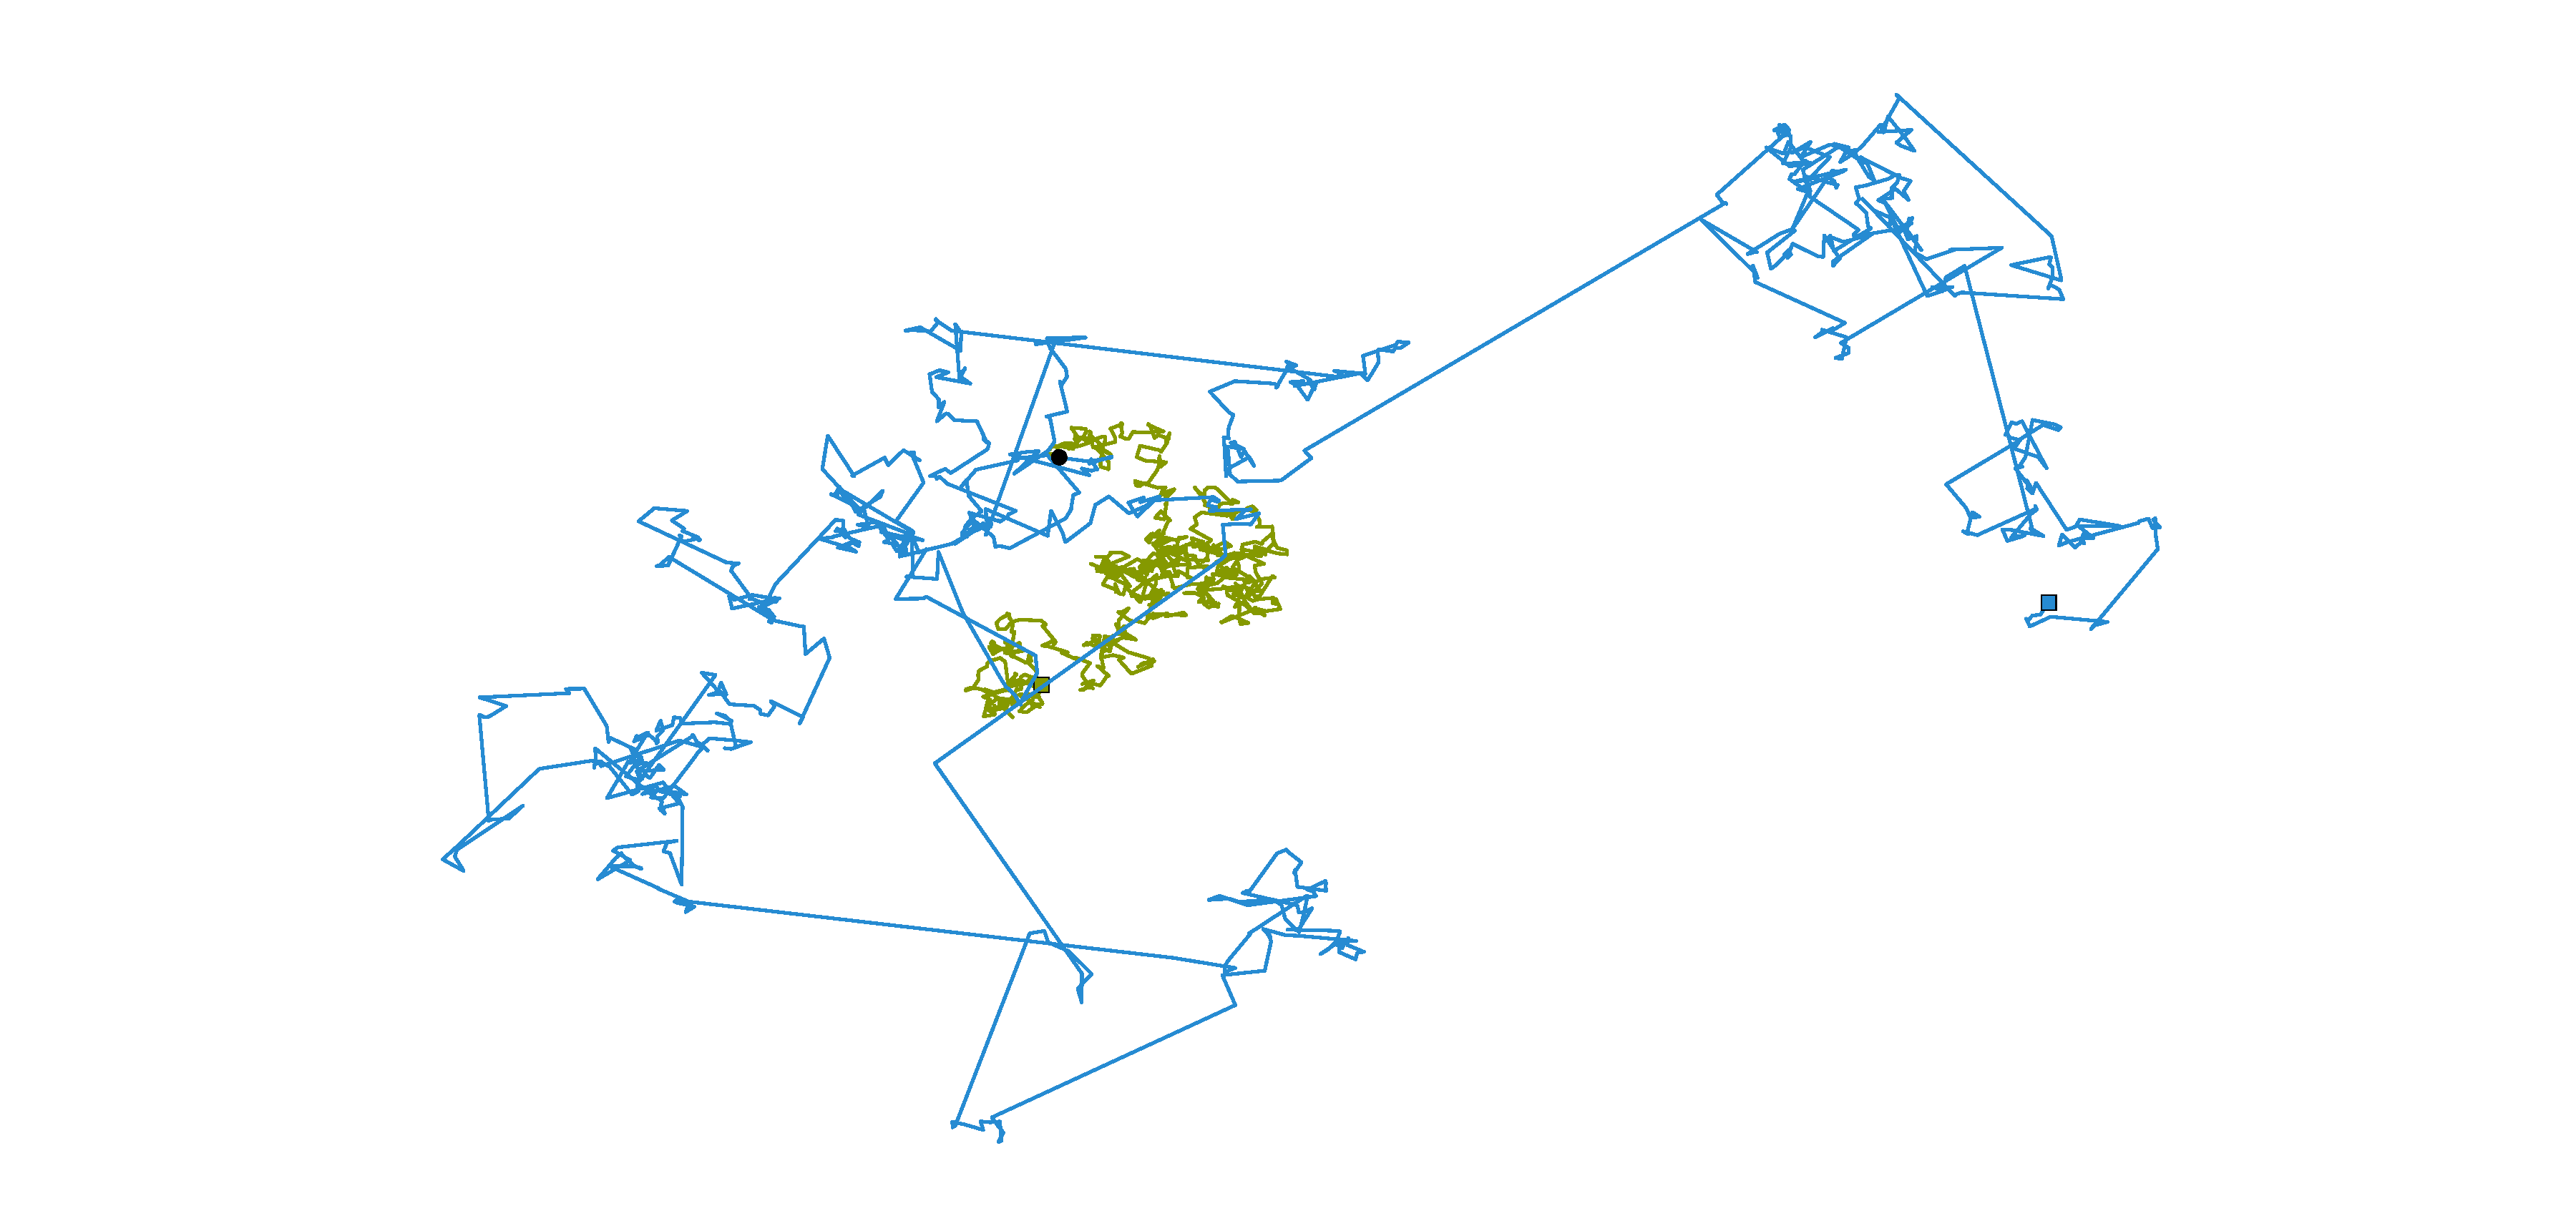
\includegraphics{LevyFlight/levy_vs_gaussian.pdf}
    \end{center}
    \caption{Mouvement brownien (en vert) et vol de Lévy (en bleu) pour 200 pas aléatoires.
             \label{fig:levy_vs_gaussian}}
\end{figure}
\FloatBarrier
% subsection vol_de_levy (end)


% ------------------------------------------------------------------------------
\subsection{Apprentissage par vecteur opposé} % (fold)
\label{sub:apprentissage_par_vecteur_oppose}
Les méthodes d’optimisation et spécifiquement les méthodes approchées sont fortement
dépendantes de la population initiale (\mtodo{Ajouter source}). Il est ainsi nécessaire
de constituer une population couvrant de manière homogène l’espace de décision.
L’approche la plus répandue consiste à construire une population initiale stochastiquement
à l’aide d’une distribution uniforme suivant \eqref{alg:init_phase}.
Afin d’améliorer la diversité / qualité de la population initiale sans connaissance
a priori, \textcite{Tizhoosh2005695} a développé l’apprentissage par vecteur opposé
(\textit{OBL} pour Opposite Based Learning) (Définition\ref{def:oblm}).

\begin{Def}[OBL~:~Apprentissage par vecteur opposé]\label{def:oblm}
Admettons un position de dimension $D$, $\vec{x}(x_{1}, x_{2}, ..., x_{D})$ avec
$x_{1}, x_{2}, ..., x_{D}$ des valeurs bornées. Si $x_{j} \in [c_{j}, d_{j}]$ pour
$j = 1, 2, ..., D$ alors la position opposée est $\vec{\check{x}}(\check{x_{1}},%
\check{x_{2}}, ..., \check{x_{D}})$ est définie par:
\[\check{x_{j}} = c_{j} + d_{j} - x_{j}\]
\end{Def}

\textcite{Rahnamayan2008906} l’adaptent pour l’algorithme Differential Evolution (\textit{DE})
et montrent que la probabilité d’améliorer une solution est plus grande si on sélectionne
la position opposée que si on tire aléatoirement une autre position.
Dans leur implémentation, ils l’utilisent durant l’initialisation mais aussi au cours du
processus d’optimisation. Les bornes ($c_{j}$ et $d_{j}$) sont alors définies dynamiquement
afin d’éviter de ralentir la convergence.
Cette approche a aussi été appliquée avec succès dans le cas de l’algorithme \textit{ABC}
en association avec un opérateur de mutation \parencite{Bi2011174}, ou encore en coopération
avec une marche aléatoire \parencite{Sharma2012213}. Elle a aussi été utilisée pour
résoudre des problèmes à objectifs multiples, en combinaison avec un algorithme
évolutionnaire \parencite{Ma201448}, ou encore avec le \textit{PSO} \parencite{Gao2013114}.

L’approche est ainsi retenue afin d’améliorer la diversité de la population initiale
et sera aussi utilisée durant la phase des exploratrices afin d’augmenter la qualité
de la nouvelle position.
Pour chaque source, une position candidate ($\vec{x}$) et son opposée
($\vec{\check{x}}$) sont ainsi évaluées. Une sélection par tournoi binaire permet
de retenir la meilleure des deux comme nouvelle position pour la source.
% subsection apprentissage_par_vecteur_oppose (end)


\subsection[L’epsilon-dominance]{L’$\epsilon$-dominance} % (fold)
\label{sub:l_epsilon_dominance}
Contrairement à une approche mono-objectif, il existe plusieurs solutions optimales
dans une approche multi-objectif. Il apparaît alors nécessaire de conserver l’évolution
du front de \textit{Pareto}~: c’est le rôle de l’archive \parencite{Laumanns2002263}.

Afin de garantir la convergence, il est nécessaire d’utiliser une approche élitiste
en limitant la population de l’archive aux solutions les plus performantes \parencite{Zitzler2000173}.
De plus, afin d’éviter de converger vers un front local, la population doit conserver
une bonne diversité.
L’algorithme de base du \textit{NSGA-II} \parencite{Deb2002182}, utilise le \textit{Fast
Non Dominated Sorting Algorithm} afin de construire son archive. Dans cette approche une
sélection par rang est appliquée afin de trier les solutions en différents niveaux et la
distance dite de crowding (distance moyenne entre deux solutions) est utilisée afin de
maintenir la diversité. L’algorithme \textit{SPEA II} cherche à améliore la diversité du
front final au prix d’une convergence plus lente en utilisant une approche par clustering.
Dans cette approche la taille limite de l’archive est définie par le nombre de cluster.
Ces clusters sont formés en se basant sur la distance euclidienne et une seule solution
est retenue.
\textcite{Laumanns2002263} proposent une autre approche, séparer l’espace des solutions en une
grille dont les dimensions sont définies par le vecteur $\vec{\epsilon}$. Dans cette
approche l’espace des objectifs est divisé en hypercubes, et chaque hypercube est comparé
selon l’$\epsilon$-dominance (Définition\ref{def:eps_dominance}). Bien que d’autres
approches utilisent une grille similaire (PAES) \parencite{Knowles2000149},
l’$\epsilon$-dominance n’accepte qu’une unique solution par hypercube assurant une plus
grande diversité de la population. La taille de l’archive est donc fonction des $\epsilon$
choisis pour chaque objectif et est donc toujours garanti d’être finie.


\begin{Def}[$\epsilon$-dominance]\label{def:eps_dominance}
L’$\epsilon$-dominance assume que deux solutions sont identiques lorsqu’elles appartiennent
au même hypercube dont les dimensions des arrêtes sont définies par
$\vec{\epsilon}_{m}, m \in \{1, ..., M\}$ avec $M$ le nombre de fonctions objectif.
Dans le cas d’une maximisation il est dit que $\vec{x}_{a}$ $\epsilon$-domine $\vec{x}_{b}$ si~:
\begin{align*}
  \forall m \in \{1, M\}, \qquad
  \left\lceil\frac{f_{m}(\vec{x}_{a})}{\epsilon}\right\rceil &\leq
  \left\lceil\frac{f_{m}(\vec{x}_{b})}{\epsilon}\right\rceil  \\
  \intertext{et}
  \exists m \in \{1, M\}, \qquad
  \left\lceil\frac{f_{m}(\vec{x}_{a})}{\epsilon}\right\rceil &<
  \left\lceil\frac{f_{m}(\vec{x}_{b})}{\epsilon}\right\rceil  \\
\end{align*}
Cette relation sera notée sera notée~: $\vec{x}_{a} \prec_{\epsilon} \vec{x}_{b}$.
\end{Def}

Une solution peut ainsi être ou dominée, dominante, identique, ou non-dominée au sens de
l’$\epsilon$-dominance, les solutions $\epsilon$-non-dominées formant alors le front
d’$\epsilon$-Pareto (Fig.~\ref{fig:epsilon_dominance}). Lors de l’ajout d’une solution à
l’archive l’$\epsilon$-dominance est alors utilisée dans un premier temps afin de les
départager. Dans le cas où la nouvelle solution serait $\epsilon$-identique elle est
uniquement comparée avec celle déjà archivée dans le même hypercube. La distance
euclidienne est alors utilisée pour les départager. La solution retenue est celle la plus
proche de l’optimum de l’hypercube (coin supérieur droit dans le cas d’une maximisation).
Contrairement à une sélection par dominance stricte le calcul de la distance euclidienne
permet de tenir compte de l’ensemble des amélioration et est moins élitiste. Afin d’éviter
l’ajout de biais, les objectifs sont normalisés dans l’espace de l’hypercube.
L’$\epsilon$-archive permet ainsi d’assurer~:
\begin{itemize}
  \item L’élitisme~: seule les solutions non-dominées sont retenues
  \item La diversification~: une unique solution par hypercube
  \item Une taille limite~: La taille maximale est fonction de $\vec{\epsilon}$ et est finie
  \item Une intensification~: En réduisant $\vec{\epsilon}$ on augmente la taille maximale de l’archive
  \item Une réduction~: En augmentant $\vec{\epsilon}$ on réduit la taille maximale de l’archive
\end{itemize}

\begin{figure}
    \begin{center}
        \includegraphics{Ressources/Images/abc/selection_boxes.pdf}
    \end{center}
    \caption{Principe de la mise à jour de l’archive par epsilon-dominance (maximisation assumée).
             Adapté de \cite{Deb2005501}.
             \label{fig:epsilon_dominance}}
\end{figure}
L’étude réalisée par \textcite{Deb2005501} montre que l’$\epsilon$-dominance permet
d’obtenir une très bonne convergence et une grande diversité sur le front final.
Les résultats indiquent que les approches \textit{PESA} et \textit{NSGA II} obtiennent une moins
bonne représentation du front de Pareto que celles utilisant l’$\epsilon$-dominance
(\textit{$\epsilon$-MOEA}) ou le clustering (\textit{C-NSGA II}, \textit{SPEA}).
Cette observation est d’autant plus vraie pour des problèmes ayant plus de deux
objectifs (\textit{DTLZ1}, ..., \textit{DTLZ7}).
De plus les résultats mettent aussi en évidence que le \textit{NSGA II} et le \textit{$\epsilon$-MOEA}
convergent plus rapidement que le \textit{SPEA II}.
Un désavantage à cette méthode peut cependant être noté. De part sa formulation
les solutions au niveau des extrêmes sur le front de Pareto sont plus difficilement
atteignables.

L’$\epsilon$-archive est donc retenue comme solution d’archivage dans ces travaux
car il représente un bon compromis entre diversité et convergence.
% subsection l_epsilon_dominance (end)


% ------------------------------------------------------------------------------
\subsection{Tenir compte des contraintes} % (fold)
\label{sub:tenir_compte_des_contraintes}
Les problèmes multi-objectif dans le domaine de l’ingénierie sont souvent
dépendants de contraintes limitant l’ensemble des solutions optimales au domaine
de faisabilité. L’optimisation consiste alors à améliorer les objectifs tout en
respectant les contraintes spécifiques au problème \eqref{eq:def_optimisation}.

La littérature introduit de nombreuses méthodes permettant de tenir compte des
contraintes. L’approche la plus courante est d’utiliser un facteur de pénalité. Ce facteur
est dit statique si il est fixe durant l’ensemble de l’optimisation, dynamique si il est
adapté en fonction du nombre d’itération, et adaptatif si les informations acquises par la
recherche aide à sa détermination \parencite{Coello2002}. Parmi les approches existantes il
peut être cité la méthode de la peine de mort. Elle consiste à appliquer une pénalité très
importante aux objectifs afin de rejeter toutes les solutions sous contraintes. Certaines
moins exclusives désavantagent les solutions ne respectant pas les contraintes en fonction
de leur niveau de violation alors que d’autres ajustent dynamiquement la pénalité en
fonction du nombre d’itérations déjà réalisées. Le problème récurrent avec ces approches
réside dans l’ajout de paramètres supplémentaires qui doivent être déterminés empiriquement.

\textcite{Coello2002} explique qu’une bonne prise en compte des contraintes ne devraient
pas nécessiter le paramétrage de facteurs car ils impactent
fortement la performance de la méthode. Finalement, la méthode sélectionnée ne
doit pas nécessiter un nombre plus important d’évaluations car elles peuvent être coûteuses.
\textcite{Deb2000311} propose une méthode de sélection par tournoi respectant ces conditions
dont les règles sont les suivantes~:
\begin{itemize}
  \item Une solution avec contraintes est inférieure à une solution sans contraintes
  \item Si les deux solutions sont sans contraintes la solution dominante est préférée
  \item Si les deux solutions sont sous contraintes, la solution violant le moins les contraintes est préférée
\end{itemize}
La méthode a l’avantage d’être simple à mettre en place mais est cependant
très élitiste car les solutions non faisables sont toujours écartées durant la
recherche.

Dans ces travaux, une méthode adaptative moins élitiste est retenue. Adaptée
aux problèmes multi-objectif par \textcite{Woldesenbet20073077}, la méthode ne demande
aucun paramétrage, et l’objectif modifié est calculé de la manière suivante~:
\begin{itemize}
  \item Normaliser les objectifs selon \eqref{eq:norm_obj}
  \item Normaliser les contraintes et les agréger pour former une unique contrainte selon \eqref{eq:norm_contrainte}
  \item Calculer les objectifs modifiés par agrégation des contraintes et des objectifs selon \eqref{eq:calc_modif_obj}
\end{itemize}

\begin{align}\label{eq:norm_obj}
  \tilde{f}_{m}(\vec{x}) &= \begin{cases}
    \frac{f_{m}(\vec{x}) - min(f_{m}(\vec{x}))}{max(f_{m}(\vec{x})) - min(f_{m}(\vec{x}))}
    & \text{(minimisation)} \\ \\ 1 - \left[\frac{f_{m}(\vec{x}) -
    min(f_{m}(\vec{x}))}{max(f_{m}(\vec{x})) - min(f_{m}(\vec{x}))}\right] &
    \text{(maximisation)} \\
  \end{cases}
\end{align}
avec $f_{m}(\vec{x})$ la valeur de l’objectif $m$, pour la position $\vec{x}$ dans l’espace de décision.

\begin{equation}\label{eq:norm_contrainte}
  v(\vec{x}) = \frac{1}{Q} \sum_{q=1}^{Q} \left(\frac{g_{q}(\vec{x})}{max(g_{q}(\vec{x}))}\right)
\end{equation}
avec $Q$ le nombre de contraintes d’inégalités. $g_{q}$ représente alors la fonction contrainte
associée à la contrainte $q$ avec $g_{q} \geq 0$. Dans cette représentation les contraintes
d’égalité doivent être transformées en contraintes d’inégalité.

\begin{equation}\label{eq:calc_modif_obj}
  F_{m}(\vec{x}) = d_{m}(\vec{x}) + p_{m}(\vec{x})
\end{equation}
avec $d_{m}(\vec{x})$ calculée selon \eqref{eq:dist_obj} et $ p_{m}(\vec{x})$ selon \eqref{eq:penalty_norm}.


\begin{align}\label{eq:dist_obj}
  d_{m}(\vec{x}) = \begin{cases}
                          v(\vec{x})                                     & \qquad si\  r_{f} = 0 \\
                          \sqrt{v(\vec{x})^2 + \tilde{f}_{m}(\vec{x})^2} & \qquad sinon          \\
                    \end{cases}
\end{align}
\begin{equation}\label{eq:penalty_norm}
  p_{m}(\vec{x}) = (1 - r_{f})  X(\vec{x}) + r_{f} Y_{m}(\vec{x}) \\
\end{equation}

\begin{align*}
  \shortintertext{où} \\
    r_{f} &= \frac{\text{Nombre de solution réalisables}}{\text{Taille de la population}} \\
  \shortintertext{et} \\
  X(\vec{x})     &= \begin{cases}
                0,          \qquad     & si\  r_{f} = 0\\
                v(\vec{x}), \qquad     & sinon\\
                \end{cases} \\
  Y_{m}(\vec{x}) &= \begin{cases}
                    0,          \quad \qquad & \text{si} \ \forall q, \ g_{q}(\vec{x}) = 0\\
                      \tilde{f}_{m}(\vec{x})  \\
            \end{cases}\\
\end{align*}

L’algorithme s’adapte ainsi dynamiquement à la population et peut accepter des
solutions ne respectant pas les contraintes. Plus il y a de solutions non
réalisables dans la population, moins une solution ne respectant pas les contraintes à
de chances d’être sélectionnée. L’approche permet d’améliorer l’exploration de
l’espace de décision et ainsi de pouvoir trouver des solutions existantes même
lorsque l’espace de faisabilité est faible.
L’approche est donc retenue dans ces travaux afin de mettre à jour la position des
sources, les solutions retenues dans l’archive doivent elles respecter
l’ensemble des contraintes pour être acceptées.
% subsection tenir_compte_des_contraintes (end)


% ------------------------------------------------------------------------------
\subsection{Description de l’approche globale} % (fold)
\label{sub:description_de_l_approche_globale}
Dans la section précédente, chaque élément utilisé dans l’algorithme a été détaillé et
les avantages et inconvénients des approches retenues ont aussi été explicités.
Dans cette section le fonctionnement global de la méthode approchée d’optimisation
multi-objectif retenue est décrit.

L’algorithme peut être définie par Fig.~\ref{fig:abc_complet}.
Les sources sont initialisées (Algorithm~\ref{alg:init_phase}) suivant la méthode
\textit{OBL} (Définition\ref{def:oblm}) afin d’obtenir une meilleure représentation du
domaine de décision en amont de l’optimisation.
Durant la phase des butineuses (Algorithm~\ref{alg:employed_phase}), chaque source
subit une variation en tenant compte de deux sources, une de l’essaim et une de l’archive.
Durant la phase des ouvrières (Algorithm~\ref{alg:onlooker_phase}), la qualité de
chaque source \eqref{eq:attribution_prob_to_source} est utilisée afin de sélectionner
et d’exploiter seulement les plus prometteuses. Finalement, si une source a été
modifiée infructueusement plus de $MaxEchec$, alors une exploratrice
réinitialise sa position de manière aléatoire  (Algorithm~\ref{alg:scout_phase}).
Tant que la condition d’arrêt n’est pas atteinte, les phases des butineuses,
des ouvrières, et des exploratrices sont répétées de manière cyclique. Au cours de
la recherche les nouvelles sources sont ajoutées à l’archive et sont utilisées
comme élément d’apprentissage pour les abeilles butineuses ou ouvrières. Les
exploratrices, elles, n’utilisent jamais d’élément sociaux d’apprentissage.
Finalement, une fois la condition d’arrêt atteinte l’ensemble des solutions
de l’archive forme le front de Pareto.

\begin{figure}
    \begin{center}
        \includegraphics[width=10cm]{abc/algorithme_complet.pdf}
    \end{center}
    \caption{Description globale de l’algorithme ABC pour les problèmes multi-objectif.
             \label{fig:abc_complet}}
\end{figure}

Dans l’optique de l’optimisation d’un modèle solaire développé sous \textit{Dymola}, l’algorithme
a été implémenté en \textit{Python} afin de faciliter le couplage avec la bibliothèque
\textit{BuildingsPy} qui comme nous l’avons vu dans le chapitre précédent permet d’automatiser
la simulation de modèle \textit{Modelica} sous \textit{Dymola}. La bibliothèque est
disponible sous le nom de \textit{pyMOABC} et implémente~:
\begin{itemize}
  \item Une $\epsilon$-archive et la hypercube-dominance
  \item La dominance au sens de Pareto
  \item La prise en compte des contraintes suivant la méthode de \textcite{Woldesenbet20073077}
  \item Une interface commune permettant l’abstraction du type de variable (discrète, continue, qualitative)
  \item Une représentation des solutions (sources et abeilles)
  \item L’algorithme tel que décrit dans ces travaux
  \item Une suite de test unitaires et des cas théorique validant l’approche avec
        et sans contraintes
\end{itemize}

L’approche retenue contrairement à la majorité des méta-heuristiques demande
peu de paramètre à définir de manière empirique et est ainsi robuste. En effet
seule la taille de la population $NP$, et le nombre d’essai maximum $MaxEchec$ sont à définir.
De plus la taille de la population n’impacte pas le nombre de solutions dans l’archive
car le stockage est réalisé dans une structure indépendante. Il est aussi important
de noter que les deux uniques paramètres on un comportement prévisible facilitant
leur paramétrage. La taille de la population en augmentant améliore l’exploration
réduisant les risques de stagner vers des optimums locaux mais réduit la vitesse
de convergence (Définition\ref{def:convergence}).
Le nombre d’essai maximum lui est directement lié au nombre de variable de décision
et à la taille de la population. Une valeur faible se traduit par un abandon rapide
des solutions alors qu’une valeur plus grande augmente le nombre de variations évaluées
pour chaque source. Ainsi on note clairement l’impact de chaque paramètre sur la
performance de l’algorithme simplifiant sa paramétrisation.

% Phase d’initialisation
\begin{algorithm}\label{alg:init_phase}
  \SetAlgoVlined
  \DontPrintSemicolon
  \emph{Initialisation des \ASources sur l’ensemble de l’espace de décision}\;
  \For{$i \leftarrow 0$ \KwTo \ANbrSources}
  {
    \emph{Initialisation des variables de décision pour chaque source}\;
    \For{$j \leftarrow 0$ \KwTo \ANbrVariables}
    {
      \encircle{a} \emph{Initialisation de la position de la $\ASource_{i}$ de manière aléatoire}\;
      \Indp
      $x_{ij} = x_{j}^{min} + RandUniform(0, 1) \times (x_{j}^{max} - x_{j}^{min})$\;
      \Indm
      \BlankLine
      \encircle{b}  \emph{Génération de l’$\ABee_{i}$ dont la position est générée suivant Définition\ref{def:oblm}}\;
      \Indp
      $ \check{x_{ij}} = x_{j}^{min} + x_{j}^{max} - x_{ij}$\;
      \Indm
      \BlankLine
      \encircle{c} \emph{Évaluation de la $\ASource_{i}$ et de l’$\ABee_{i}$}\;
      \BlankLine
      avec $RandUniform$ un tirage aléatoire suivant une loi uniforme, et $x_{j}^{min}$, $x_{j}^{max}$
      respectivement le minimum et le maximum de la variable $j$\;
    }
    \If{$\ASource_{i}$ respecte toutes les contraintes}
    {
      $\AArchive \pluseq \ASource_{i}$ \AComment{On ajoute la source initial à l’archive}
    }
    \If{$\ABee_{i}$ respecte toutes les contraintes}
    {
      $\AArchive \pluseq \ABee_{i}$ \AComment{On ajoute la source opposée à l’archive}
    }
  }
  Mise à jour des \ASources d’après Algorithm~\ref{alg:maj_phase}\;
  \caption{Initialisation des sources par OBLM (Définition\ref{def:oblm}).}
\end{algorithm}

% Phase des éclaireuses
\begin{algorithm}\label{alg:scout_phase}
  \SetAlgoVlined
  \DontPrintSemicolon
  \AComment{Exploration par les \AScouts}
  \For{$i \leftarrow 0$ \KwTo \ANbrSources}
  {
    \If{$\ATrial_{i} > \AMaxTrial$ }
    {
      Génération de deux nouvelles positions suivant Algorithm~\ref{alg:init_phase}\;
    }
  }
  Mise à jour de la position des \ASources d’après Algorithm~\ref{alg:maj_phase}\;
  \caption{Phase des éclaireuses.}
\end{algorithm}


% Phase des ouvrières
\begin{algorithm}\label{alg:onlooker_phase}
  \SetAlgoVlined
  \DontPrintSemicolon
  \AComment{Exploitation des sources par les \AOnlookers}
  \AComment{Plusieurs \AOnlookers peuvent modifier la même source}
  \For{$\AOuvriere \in \AOnlookers$}
    {
      Sélection aléatoire d’une \ASource $i$ selon la probabilité
      définie par l’équation \eqref{eq:attribution_prob_to_source}\;
      Sélection aléatoire d’une source $a$ ($a \neq i$) dans l’\AArchive\;
      \encircle{a} \emph{Génération d’une nouvelle position $\vec{x_{i}}'$ à partir de la
                         position $\vec{x_{i}}$ pour l’\AOuvriere }\;
      \For{$j \leftarrow 0$ \KwTo \ANbrVariables}
      {
      \begin{algomathdisplay}
        x_{ij}' =%
          \begin{cases}
            x_{ij}  + RandUniform(-1, 1)   \times \ (x_{ij} - x_{aj}) &\ \ATirageB < \AMR \\
            x_{ij}                                                    &\ sinon
          \end{cases}
      \end{algomathdisplay}
      }
      \BlankLine
      Avec \AMR est la probabilité de réaliser une modification (fixée à 0,2) et
      \ATirageB un nombre aléatoire entre 0 et 1\;
      \BlankLine
      \encircle{b} \emph{Évaluation des objectifs pour la nouvelle position $\vec{x_{i}}'$}\;
      \BlankLine
      \If{\AOuvriere respecte toutes les contraintes}
      {
        $\AArchive \pluseq \AOuvriere$ \AComment{Ajout de la solution trouvée par l’\AOuvriere à l’archive}
      }
    }

  Mise à jour de la position des \ASources qui ont été modifiées d’après Algorithme~\ref{alg:maj_phase}\;
  \caption{Phase des ouvrières.}
\end{algorithm}

% Maj des sources
\begin{algorithm}\label{alg:maj_phase}
  \SetAlgoVlined
  \DontPrintSemicolon
  Récupérer le maximum et minimum pour chaque objectif dans l’\AHive\;
  Récupérer le maximum pour chaque contrainte dans l’\AHive\;
  \For{$\ABee \in \ABees$}
  {
    Calcul du vecteur objectif pour l’\ABee ($\vec{F}'_{i}$) et pour sa \ASource $i$ ($\vec{F}_{i}$),
    respectivement aux positions $\vec{x_{i}}'$ et $\vec{x_{i}}$
    selon \eqref{eq:calc_modif_obj}\;
    \For{$m \leftarrow 1$ \KwTo M}
    {
      \begin{algomathdisplay}
      \begin{aligned}
      F_{im}' &= d_{m}'(\vec{x_{i}}) + p_{m}'(\vec{x_{i}}) \\
      F_{im}  &= d_{m}(\vec{x_{i}}) + p_{m}(\vec{x_{i}})   \\
      \end{aligned}
      \end{algomathdisplay}
    }
    \If{$\vec{x_{i}}' \succ \vec{x_{i}}$}
    {

      $\ASource_{i} \leftarrow \ABee$ \AComment{Mise à jour de la \ASource à partir de l’\ABee}

      $\ATrial_{i} \leftarrow 0$ \AComment{On réinitialise le nombre d’essais pour la \ASource $i$}
    }
    \Else
    {
      $\ATrial_{i} \pluseq 1$ \AComment{On incrémente le nombre d’essais pour la \ASource $i$}
    }
  }
  \caption{Mise à jour des \textbf{Sources} par les \textbf{Abeilles}}
\end{algorithm}

% Phase des butineuses
\begin{algorithm}\label{alg:employed_phase}
  \SetAlgoVlined
  \DontPrintSemicolon
  \AComment{Exploration des sources par les \AEmployed}
  \For{$i \leftarrow 0$ \KwTo \ANbrSources}
  {
    Sélection aléatoire d’une source $a$ ($a \neq i$) dans l’\AArchive\;
    Sélection aléatoire d’une source $b$ ($b \neq i$) dans l’\AHive\;
    \BlankLine
    \encircle{a} \emph{Génération d’une nouvelle position $\vec{x_{i}}'$ à partir de la %
                       position $\vec{x_{i}}$ pour la \AButineuse $i$}\;
    \If{$\ATirageA < \ARatio $ }
      {
      \For{$j \leftarrow 0$ \KwTo \ANbrVariables}
      {
      \begin{algomathdisplay}
        x_{ij}' =%
          \begin{cases}
            \begin{aligned}
              x_{ij}  &+ 0.01 \times  \ALevy  &\times \ (x_{ij} - x_{bj})  \\
                      &+ 0.01 \times |\ALevy| &\times \ (x_{aj} - x_{ij})  \\
            \end{aligned} &\ \ATirageB < \AMR \\
            x_{ij}        &\ sinon
          \end{cases}
      \end{algomathdisplay}
      \ALevy est nombre aléatoire dans une distribution de Lévy
      permettant de réaliser un vol de Lévy (Définition\ref{def:vol_levy})\;
      }
      }
    \Else
      {
      \For{$j \leftarrow 0$ \KwTo \ANbrVariables}
      {
      \begin{algomathdisplay}
        x_{ij}' =%
          \begin{cases}
            \begin{aligned}
              x_{ij}  &+ RandUniform(-1, 1)   &\times \ (x_{ij} - x_{bj})  \\
                      &+ RandUniform(0, 1)    &\times \ (x_{aj} - x_{ij})  \\
            \end{aligned} &\ \ATirageB < \AMR \\
            x_{ij}        &\ sinon
          \end{cases}
      \end{algomathdisplay}
      }
      }
      Où \ARatio est la probabilité de réaliser un vol de Lévy (fixée à 0,5), et \AMR la probabilité
      de réaliser une modification (fixée à 0,3). \ATirageA et \ATirageB étant des nombres aléatoires
      (entre 0 et 1) tirés dans une distribution uniforme\;
      \BlankLine
    \encircle{b} \emph{Évaluation des objectifs pour la nouvelle position $\vec{x_{i}}'$}\;
    \If{$\AButineuse_{i}$ respecte toutes les contraintes}
    {
      \AComment{On ajoute la nouvelle source à l’archive}
      $\AArchive \pluseq \AButineuse_{i}$\;
    }
  }
  \AComment{On ne conserve que une seule position par source}
  Mise à jour de la position des \ASources d’après Algorithme~\ref{alg:maj_phase}\;
  \caption{Phase des butineuses.}
\end{algorithm}
\FloatBarrier
% subsection description_de_l_approche_globale (end)


% ------------------------------------------------------------------------------
\subsection{Validation de la méthode} % (fold)
\label{sub:validation_de_la_methode}

\itodo{CETTE SECTION EST EN CONSTRUCTION}

Cette section permet d’apprécier la performance de l’approche pour différent types
de problèmes pouvant être rencontrés dans un problème d’optimisation.

La bibliothèque \textit{pyMOABC} a été développée autour de tests unitaires
(Test-driven development).
Chaque éléments (fonction / méthodes / ...) et comportements (minimisation / maximisation / ...)
ont ainsi été testés afin de garantir que la bibliothèque implémente correctement
les éléments et comportements nécessaires. De part son approche, chaque nouvelle
modification tient implicitement compte des tests précédents et garantie ainsi
l’intégrité du code lors de son développement.
L’algorithme et les briques nécessaires implémentés, des problèmes étalons ont été
utilisés afin de valider la performance de l’approche. Bien que la réussite d’un
problème étalon ne soit pas une condition suffisante pour garantir la convergence
sur un problème réel, il apporte une information importante~: la capacité de
l’algorithme à s’adapter aux différents types de contraintes pouvant survenir.

Dans cette optique les résultats présentés dans cette section sont sélectionnés
afin de couvrir les principales difficultés existantes~:
\begin{itemize}
  \item front convexe~: ZDT1 (2 objectifs)
  \item front linéaire~: Hanne 1 (2 objectifs)
  \item front concave~: ZDT2 (2 objectifs)
  \item multi-modal~: ZDT4 (2 objectifs)
  \item Non-uniformité avec faible densité près de l’optimal~: DTLZ5 (3 objectifs), ZDT6, ConvexGlobalNonConvexLocalHive
  \item Discontinue~: DTLZ6 (3 objectifs), Kursawe
\end{itemize}
La validation portera ainsi sur la capacité de l’algorithme à converger vers le
front de Pareto ainsi que la qualité des solutions obtenues à travers l’évaluation
de sa diversité. De plus la vitesse de convergence vers le front sera aussi discutée.
Concernant la méthode de prise en compte des contraintes, des travaux ont déjà
évalué sa performance et ces résultats ne seront pas repris dans cette section (\mtodo{Ajouter ref}).

\itodo{Ajout de graphe de convergence, et les résultats du calcul des indicateurs
       évaluant la diversité, la rapidité, et la convergence.}
% subsection validation_de_la_methode (end)
% section algorithme_de_colonie_d_abeilles_virtuelles (end)
